%xhversion{v2.01 RdF} %PdJ,PdL,PdM,PdS,PdU,Pe6,PeI,PfB,PfD,RbN,RbP,RcL,RdC,RdD,RdF
%%%%%%%%%%%%%%%%%%%%%%%%%%%%%%%%%%%%%%%%%%%%%%%%%%%%%%%%%%%%%%%%%%%%%%%%%%%%%
%	TODO:
%	-Überarbeitung des Blockschaltbildes
%	-MOVE Klasse
%	-Wie funktioniert der LAN-Modus
%	-AI-Möglichkeiten
%	-Verwendete AI
%	-Code-AI
%%%%%%%%%%%%%%%%%%%%%%%%%%%%%%%%%%%%%%%%%%%%%%%%%%%%%%%%%%%%%%%%%%%%%%%%%%%%%
%%%%%%%%%%%%%%%%%%%%%%%%%%%%%%%%%%%%%%%%%%%%%%%%%%%%%%%%%%%%%%%%%%%%%%%%%%%%%
%	die auskommentierten 'usepackage'-Anweisungen sind
%	Alternativen oder Zusaetze, die iXH hier nicht,
%	aber vielleicht DU brauchen kannst - XH
%%%%%%%%%%%%%%%%%%%%%%%%%%%%%%%%%%%%%%%%%%%%%%%%%%%%%%%%%%%%%%%%%%%%%%%%%%%%%
%	XH Herstellungsprozess-Shellscript @15Apr17:
%	--------------------------------------------
%	#!/bin/sh
%	ifn="MeinLatexFile.tex"
%	latex $ifn
%	fn2="$(echo $ifn|sed s/.tex/.dvi/)"
%	fn3="$(echo $ifn|sed s/.tex/-pics.pdf/)"
%	  ### now dvipdf  $fn2 into $fn3 Container ...
%	dvipdf $fn2  $fn3
%	#dvipdf $(echo $ifn|sed s/.tex/.dvi/)
%	  ### now pdflateXing $ifn ... (zweimal - fuers Inhaltsverzeichnis)
%	pdflatex $ifn
%	pdflatex $ifn
%%%%%%%%%%%%%%%%%%%%%%%%%%%%%%%%%%%%%%%%%%%%%%%%%%%%%%%%%%%%%%%%%%%%%%%%%%%%%
\listfiles			%lists included files while processing 'pdflatex'
  %\documentclass[12pt,a4paper]{book}
  %\documentclass[11pt,a4paper]{article}
\documentclass[12pt,a4paper]{article}
  %\documentclass[12pt,a4paper]{report}

  %\usepackage{etex}		%gegen 'no more room for new dimen...' error xh@RaE1

	% encoding:
  %%\usepackage[latin1]{inputenc}
  %%\usepackage[ansinew]{inputenc}
  %%\usepackage[cp850]{inputenc}
  %\usepackage[utf8x]{inputenc}
\usepackage[utf8]{inputenc}
\usepackage[ngerman]{babel}
\usepackage[T1]{fontenc}  %\usepackage{amssymb}
\usepackage{amsmath}
%\usepackage{extarrows}	%\xleftrightarrow[obentext]{untentext}
\usepackage{wasysym}
\usepackage{pxfonts}
\usepackage{verbatim}
\usepackage{alltt}
\usepackage{moreverb}
\usepackage{graphicx}
\usepackage{wrapfig}
\usepackage{subfigure}
\usepackage{hyperref}
\usepackage{nameref}
  %\usepackage{theorem}
  %\usepackage[dvips]{color}
  %\usepackage{lmodern}
  %\usepackage{textcomp}
\usepackage{multicol}		% 2-, 3-, ... -spaltige Formatierung mit 'multicols'
\usepackage{multirow}		% fuer 'tabular' - Tabellen
\usepackage{makeidx}
  %\usepackage{pdfpages}	% fuer 'includepdf' (iNimmMeistens 'includegraphics[page=1,...]')
\usepackage{mdwlist}		% f. 'compact lists' "itemize*", "enumerate*", "description*"
  %\usepackage{ulem}	... produziertma nFehler ban 'latex' run
\usepackage{longtable}		% fuer tabellen ueber mehrere Seiten
\usepackage{xcolor}
\definecolor{lightgrey}	{gray}{0.85}
\definecolor{llltgy}	{gray}{0.98}
\definecolor{lltgy}	{gray}{0.96}
\definecolor{ltgy}	{gray}{0.91}
\definecolor{grey}	{gray}{0.75}
\definecolor{dkgy}	{gray}{0.35}
\definecolor{ddkgy}	{gray}{0.17}
\definecolor{dddkgy}	{gray}{0.07}
\definecolor{blk}	{gray}{0.99}
\definecolor{lltgn}	{rgb}{0.96,1.0,0.96}
\definecolor{ltgn}	{rgb}{0.91,1.0,0.91}
\definecolor{mdgn}	{rgb}{0.7,1.0,0.7}
\definecolor{dkgn}	{rgb}{0.0,0.7,0.0}
\definecolor{ddkgn}	{rgb}{0.0,0.45,0.0}
\definecolor{dddkgn}	{rgb}{0.0,0.25,0.0}
\definecolor{mdye}	{rgb}{0.95,0.95,0.60}
\definecolor{ltye}	{rgb}{0.98,0.98,0.90}
\definecolor{lltor}	{rgb}{0.97,0.94,.87}
\definecolor{ltor}	{rgb}{0.95,0.85,.66}
\definecolor{red}	{rgb}{1.0,0.0,0.0}
\definecolor{dkred}	{rgb}{0.8,0.0,0.0}
\definecolor{ltrd}	{rgb}{1.0,0.8,0.8}
\definecolor{ltbu}	{rgb}{0.8,0.8,1.0}
\definecolor{mdbu}	{rgb}{0.7,0.7,1.0}
\definecolor{bu}	{rgb}{0.0,0.0,1.0}
\definecolor{dkbu}	{rgb}{0.0,0.0,0.6}
\definecolor{ddkbu}	{rgb}{0.0,0.0,0.45}
\definecolor{ddkrd}	{rgb}{0.25,0.0,0.0}
\definecolor{dkrd}	{rgb}{0.70,0.0,0.0}
\definecolor{indigo}	{rgb}{0.2,0.1,0.9}


%\lstset{language=C}
%\lstset{basicstyle=\tiny}
  %\lstset{basicstyle=\small}
  %\lstset{basicstyle=\normalsize}
%\lstset{backgroundcolor=\color{lightgrey}}
%\lstset{showstringspaces=false}
%\lstset{breaklines=true}
  %\lstset{tabsize=4}
%\lstset{morecomment=[l][\color{dkgn}]{\%},%
%	morecomment=[s][\color{dkgn}]{/*}{*/}}
%\lstset{numbers=left}

\usepackage{fancyhdr}
  %\usepackage{framed}		%'\begin{framed}' ... '\end{framed}', schautAusWiePartezettel:-)
\usepackage{hyphenat}		%fuer '\hyph{}'
  %\usepackage{lastpage}	%fuer '\pageref{LastPage}' - **funzt nid bei allen**
\usepackage{url}		%fuer '\url{...}'

% lscape oder pdflscape: ('landscape' == Querformat)
\usepackage{lscape}
  %\usepackage{pdflscape}
\usepackage{rotating}		%f. 'rotate' und 'turn'
\usepackage[active]{pst-pdf}
\usepackage{pst-circ}
\usepackage{pst-plot}
\usepackage{pst-uml}
  %\usepackage{calc}
\usepackage{fp}
  %\usepackage[official]{eurosym}
\usepackage[gen]{eurosym}

	% YHs Raender links 30mm rechts 25mm einstellen:
\setlength{\hoffset}	{30mm-1in}
\setlength{\oddsidemargin}{0pt}		%bei doppelseitigem Druck umstellen!
\setlength{\textwidth}	{\paperwidth-55mm}

%hier duerfte header Fehler liegen
\setlength{\topmargin}	{0pt}
\addtolength{\voffset}  {-16.2mm}
\addtolength{\textheight}{39mm}

\setcounter{tocdepth}{4}		%bringt auch 'paragraph{titel}' ins Inhaltsverzeichnis

\newcommand{\cmnt}[1]{}			%eigene Kommentier-Funktion \cmnt{ ...Kommentar... }
\newcommand\tbs{\textbackslash}		%'\textbackslash{}' isma z'long zan tippen ;-)
\newcommand\dtbs{\textbackslash\textbackslash}	% -dito-
%
\definecolor{ydkbu}{rgb}{0.0,0.0,0.6}	% YHs blaue Schriftfarb
\newcommand{\yhbu}[0]{\color{ydkbu}}	% Macro fuer schreibfaulen XH
\definecolor{corrclr}{rgb}{0.7,0.2,0.2}		% XHs Korrekturen-Farb ...
\newcommand{\korr}[0]{\color{corrclr}\fontsize{8pt}{9pt}\selectfont\bf} %plus Faulheitsmacro
\makeindex

	%/* Line Spacing: */
\usepackage{setspace}
% \newcommand{\mylinespacing}[0]{\singlespace}
\newcommand{\mylinespacing}[0]{\onehalfspace}	% 1,5-ZeilenAbstand
% \newcommand{\mylinespacing}[0]{\doublespace}

% /*Font Family:*/
%\renewcommand*{\familydefault}{\rmdefault}	%klassisches 'Roman' (statt MicroMurx...)
\renewcommand*{\familydefault}{\sfdefault}	%klassisches 'Helvetica' statt 'MS-Arial'


%===================================================

\usepackage{listings}
\usepackage{color}

\definecolor{dkgreen}{rgb}{0,0.6,0}
\definecolor{gray}{rgb}{0.5,0.5,0.5}
\definecolor{mauve}{rgb}{0.58,0,0.82}

\lstset{frame=tb,
  language=Java,
  aboveskip=3mm,
  belowskip=3mm,
  showstringspaces=false,
  columns=flexible,
  basicstyle={\small\ttfamily},
  numbers=none,
  numberstyle=\tiny\color{gray},
  keywordstyle=\color{blue},
  commentstyle=\color{dkgreen},
  stringstyle=\color{mauve},
  breaklines=true,
  breakatwhitespace=true,
  tabsize=3
}

%===================================================
\begin{document}
%\addtocontents{toc}{\protect\begin{multicols}{2}} %-fuer mehrspaltiges Inh.Verz




\newcommand\logoB[1]{%
	%dieses Macro '' zeichnet das "neue" HTL Logo mithilfe der
	% 'ps-tricks' Pakete/Anweisungen; Parameter#1 bestimmt die "Dicke"
	% der Balken; die "Groesse" bitte mit '\scalebox{factor}{logoB{0.12}}',
	% die Grundlinie mit '\raisebox{pos}{logoB{0.12}}' einstellen;
	% die Farbgebung spezifiziert man HIER:
  \definecolor{lobu}{rgb}{0.05,0.05,0.50}
  \definecolor{hibu}{rgb}{0.20,0.20,0.70}
  \definecolor{loye}{rgb}{0.85,0.75,0.36}
  \definecolor{hiye}{rgb}{0.99,0.92,0.00}
  \definecolor{logn}{rgb}{0.00,0.65,0.20}
  \definecolor{hign}{rgb}{0.00,0.79,0.30}
  \definecolor{lord}{rgb}{0.66,0.00,0.00}
  \definecolor{hird}{rgb}{0.89,0.00,0.00}%
  \resizebox{11.5mm}{!}{%
  \begin{pspicture}[showgrid=false](-1,-1)(1,1)
	\SpecialCoor	%das erlaubt PS -Berechnungen mit dem '!'; hier zur "DickenSkalierung"
	\pspolygon[linewidth=0.1pt,linestyle=none,fillcolor=lobu,fillstyle=solid]%
		(-#1, -1.00)( #1, -1.00)( 1.00, -#1)(! 1.00 #1 2 mul sub -#1)
	\pspolygon[linewidth=0.1pt,linestyle=none,fillcolor=hibu,fillstyle=solid]%
		(! 1.00 #1 2 mul sub          -#1)(! 1.00 #1 3 mul sub   0.00)%
		(! -#1         -1.00 #1 2 mul add)(-#1,-1.00)

	\pspolygon[linewidth=0.1pt,linestyle=none,fillcolor=hiye,fillstyle=solid]%
		( 1.00, -#1)( 1.00, #1)( #1, 1.00)(! #1   1.00 #1 2 mul sub)
	\pspolygon[linewidth=0.1pt,linestyle=none,fillcolor=loye,fillstyle=solid]%
		(! #1    1.00 #1 2 mul sub)(! 0.00   1.00 #1 3 mul sub)%
		(! 1.00 #1 2 mul sub   -#1)( 1.00, -#1)

	\pspolygon[linewidth=0.0pt,linestyle=none,fillcolor=hign,fillstyle=solid]%
		( #1, 1.00)( -#1, 1.00)(-1.00, #1)(! -1.00 #1 2 mul add   #1)
	\pspolygon[linewidth=0.0pt,linestyle=none,fillcolor=logn,fillstyle=solid]%
		(! -1.00 #1 2 mul add   #1)(! -1.00 #1 3 mul add    0.00)%
		(! #1    1.00 #1 2 mul sub)( #1, 1.00)

	\pspolygon[linewidth=0.1pt,linestyle=none,fillcolor=lord,fillstyle=solid]%
		(-1.00, #1)(-1.00, -#1)(-#1, -1.00)(! -#1    -1.00 #1 2 mul add)
	\pspolygon[linewidth=0.1pt,linestyle=none,fillcolor=hird,fillstyle=solid]%
		(! -#1   -1.00 #1 2 mul add)(! 0.00   -1.00 #1 3 mul add)%
		(! -1.00 #1 2 mul add    #1)(-1.00, #1)
	\NormalCoor
  \end{pspicture}%
  }%
}

\newcommand{\HtlHeader}[0]{%
	\hspace*{-11mm}%
	\raisebox{-1mm}{\logoB{0.12}}%
	%\includegraphics[width=10.3mm]{pics/logo}
	\hspace*{2mm}%
	\parbox[b]{110mm}{\flushleft
		{\fontsize{20pt}{20pt}\selectfont\bf HTL}
		{\fontsize{16.2pt}{16.2pt}\selectfont\color{teal}\bf anichstrasse}
		\\[-4.05mm]{\color{darkgray}\rule{110mm}{0.5pt}}
		\\[-2.24mm]{\fontsize{7pt}{7pt}\selectfont\color{darkgray}
			Elektronik $\cdot$ Elektrotechnik $\cdot$
			Maschinenbau $\cdot$ Wirtschaftsingenieure
			\rule{0pt}{0mm}
		%\vspace*{1.1mm}
		}
	}%
	\hspace*{5mm}%
	%\raisebox{-0.2mm}{ \includegraphics[width=25mm]{pics/HTLgenlogo02}}
	\\[-1.5mm]\rule{\textwidth}{0.5pt}
	%\hfill
}%HtlHeader







	%/* Deckblatt */
\begin{titlepage}
 \begin{center}
   \begin{minipage}{\linewidth}
   \begin{center}
   \HtlHeader{}
	\vspace*{-10mm}
	{\fontsize{25pt}{25pt}\selectfont\bf \\[10mm]\text{DIPLOMARBEIT}}
	\\[19mm]{\fontsize{20pt}{20pt}\selectfont\textbf{\textsc{JavaChess, ChessPI AndChess}}}
	\\[15mm]{\fontsize{12.4pt}{12.4pt}\selectfont\bf
		Höhere Technische Bundeslehr- und Versuchsanstalt Anichstrasse}
	\\[ 5mm]\rule{132mm}{1.0pt}
	\\[ 4mm]{\fontsize{12.4pt}{12.4pt}\selectfont\bf Abteilung}
	\\[ 5mm]{\fontsize{12.4pt}{12.4pt}\selectfont\bf Elektronik \& Technische Informatik}
	\\[24mm]{\hspace*{2mm}\parbox{154mm}{\fontsize{12.4pt}{12.4pt}\selectfont
	  \parbox[t]{75mm}{
		Ausgefuehrt im Schuljahr 2017/18 von:
		\\[5.0mm]Alexander Beiser 5CHEL
		\\[2.5mm]Marcel Huber 5CHEL 
	  }
	  \hspace*{6mm}
	  \parbox[t]{50mm}{
		Betreuer/Betreuerin:
		\\[5.0mm]Ing. MSc. Signitzer Markus
	  }
	  \\[14mm]{Innsbruck, am 30.10.2017}
	  \\[16mm]\rule{150mm}{0.5pt}
	  \\[ 8mm]
	  \parbox[t]{75mm}{
		Abgabevermerk:
		\\[3.25mm]Datum:
	  }
	  \hspace*{6mm}
	  \parbox[t]{50mm}{
		Betreuer/in:
	  }
	}}
   \end{center}\hfill
   \end{minipage}
 \end{center}
\end{titlepage}


\addtocounter{page}{1}


%====================================================================================
%Liebe LaTeXniker!
%hierher kaeme das Inhaltsverzeichnis, empfehlenswerterweise mit Seitenwechsel
%\clearpage	%erzwingt Ausdruck noch ungedruckter 'floats'
%\vfill		%fuellt die Seite mit Leerraum auf
%\newpage	%erzwingt Seitenumbruch
%\tableofcontents
%====================================================================================


	%/*Header-Einstellung*/
\pagestyle{fancy}
\fancyhf{}
\renewcommand{\sectionmark}[1]{\markright{#1}}
\renewcommand{\subsectionmark}[1]{\markright{#1}}
\renewcommand{\subsubsectionmark}[1]{\markright{#1}}
\lhead{}
\chead{\HtlHeader{}}
\rhead{}
\lfoot{Beiser/Huber}
\cfoot{\thesection-\rightmark}
%\cfoot{\thesubsubsection-\rightmark}
\rfoot[\thepage]{\thepage/\pageref{LastPage}}
\setlength{\headwidth}	{1.0\textwidth}
\setlength{\headheight}{15mm}
\renewcommand{\headrulewidth}{0.0pt}
\renewcommand{\footrulewidth}{0.33pt}


\vfill
\newpage
\tableofcontents










%====================================================================================
%Best comment of all time!!!
\cmnt{
	Hier anfangs the Document Text.
	("\cmnt" isa self written very simple Macro for Kommentare:
	\newcommand{\cmnt}[1]{ }
                      !    !  !
                      !    !  +--- what to do, here also nix
                      !    +------ number of Parameters: se Kommentar-Text
                      +----------- name of new command
	)
	
	The "\yhbu" colored Sections are Vorgaben (recommendations) by AV YH.
	All se blue Zuig have to verschwind in se final version of your Diplomschrift(DS).
	(iXH recommend not to translate the words 'Diplomschrift' or 'Diplomarbeit'
	into 'diploma document', 'diploma project' or such Kas,
	because the original words are defined in se Austrian Law, Verordnungen
	and derlei rechtlix Plunder; so it is like an Eingenname,
	which we also dont uebersetz:
	You dont traslate 'HTL' to 'UTEC' (upper technical education corporation)
	or
	'Hansi' ('H', 'ans', 'i') 'Meier' ('M' and 'eier') into 'Ageoneeye Emeggs'
	oder?? )

	("\yhbu" Macro see above; is also a selber-defined macro:
	\definecolor{ydkbu}	{rgb}{0.0,0.0,0.5}   %make a Farb-Name
	               !          !     !   !   +--- Blau-Anteil
	               !          !     !   +------- Gruen-Anteil
	               !          !     +----------- Rot-Anteil
	               !          +----------------- Farbmodell 'RGB'
	               +---------------------------- name of se new Farb
	\newcommand{\yhbu}[0]{\color{ydkbu}}  %define se new macro
	              !    !       +--------- schreib des in LaTeX-Text eini
	              !    +----------------- 0 = null parameters, also keine
	              +---------------------- name of macro
	-> "\yhbu" gets replaced by "\color{ydkbu}"
	(what does this bring?:
	you can later change se color for all se "yhbu" parts gemeinsam
	without wurschtling through the whole document;
	also wenn mir die Farb no nid gfallt, aendris uanfoch in Macro)

	You can change the
		line spacing (einzeilig, 1.5zeilig und so)
	by schreibing one of
	   \newcommand{\mylinespacing}[0]{\singlespace}
	   \newcommand{\mylinespacing}[0]{\onehalfspace}
	   \newcommand{\mylinespacing}[0]{\doublespace}
	and using '\mylinespacing' in se document preamble (=header) part
	and the
		font family
		(Roman(serif) or se ugly Arial/Helvetica(sanserif))
	writing
	   \renewcommand*{\familydefault}{\rmdefault}
	   \renewcommand*{\familydefault}{\sfdefault}
	weiter oben in se preamble (isch bei se Macos oben)

	Be free to change se Deckblatt
	and se HTL-Header (dann isches aber nimma 'der HTL-Header'! ...and YH will fauch on you)

	mirXH persoenlich gfollaz besser min HTL-Header auf jedn Blattl
	(command: \lhead{\HtlHeader})
	he ghearat holt black-and-white, because colors gelten als 'kitschig' (kitchy)
	aber me asks jo nobody (i am only a small Wuerschtl from se behindmountain (Hintelgebilge))

	ATTENTION!
	This 'Inhaltsverzeichnis'
	does NOT pass zu se document text here.
	i just gewaltsam made it look like YH's Vorlage.
	iXH also dont understand,
	why it is mitten im Dokument anstatt at se beginnig or at se end,
	why se headline (Ueberschrift) is not at it's first page oben,
	but ganz lonely on the page before,
	and why it starts with Kapitel 2.1 anstatt 1.0
	and on page 8 statt 1 oder 2;
	it suggeriers that Loesungswege, Nutzwertanalysen, Grobwentwurf, Feinentwurf
	und Implementierung auf derselben Seite 11 Platz haben,
	Fertigungsdokumentation plus Gebrauchsanweisung (S.14)
	sowie das Pflichtenheft(S.18) nur 1 Seite lang sein brauchen,
	se p.22 must be empty
	and se Projektterminplanung erst am Ende des Projektes nach der
	Feststellung der Projekterfahrungen erfolgt.
	but i am eben a dumms kind, a small Wuerschtl...


}%cmnt
%====================================================================================

\mylinespacing
{




%====================================================================================
\clearpage\vfill\newpage%\part{U-Lektionen \dq{}embedded Systems\dq{}}
%====================================================================================

\addcontentsline{toc}{section}{Erklaerung der Eigenstaendigkeit der Arbeit}
\section*{\Large\sc Erklaerung der Eigenstaendigkeit der Arbeit}
	\hfill\\[ 8mm]
	EIDESSTATTLICHE ERKLÄRUNG
	\\[3mm]
\begin{spacing}{1.5}
	\noindent%
	Ich erklaere an Eides statt, dass ich die vorliegende Diplomarbeit selbstaendig und
	ohne fremde Hilfe verfasst, andere als die angegebenen Quellen und Hilfsmittel
	nicht benutzt und die den benutzten Quellen woertlich und inhaltlich entnommenen
	Stellen als solche erkenntlich gemacht habe.
\end{spacing}\hfill
	\\[12mm]
	\parbox[b]{52mm}{
		\rule{50mm}{0.2pt}\rule{0pt}{25mm}
		\\\hspace*{6mm}{Ort, Datum}
		\\[0mm]
	}
	\hfill
	\parbox[b]{72mm}{
		\rule{70mm}{0.2pt}\rule{0pt}{25mm}
		\\\hspace*{6mm}{Verfasser, Verfasserinnen}
		\\\hspace*{6mm}{Vor- und Zunamen}
	}







%======================================================================================
%\clearpage\vfill\newpage
%======================================================================================
\newpage
\section{Zusammenfassung des Projektergebnisses}
 \subsection{Kurzfassung /Abstract}
 
	Alexander Beiser und Marcel Huber entwickelten im Zuge ihrer Diplomarbeit 2017/18 ein Schachspiel, welches auf einem PC, Android-Smartphone und Raspberry PI spielbar ist. Das Schachspiel basierte auf einem bereits von ihnen geschriebenen rohen ,,Gerüst''. \\
	Dieses Spiel wurde mit der Programmiersprache Java entwickelt, weiteres war für den Raspberry PI ein Gehäuse zu Designen und mit einem 3D Drucker zu realisieren. Um das Spielvergnügen für den Raspberry PI auch Unterwegs zu ermöglichen wurde eine Akkusteuerung entworfen und realisiert. \\
	\subsubsection{Alexander Beiser}
	Alexander Beiser war für große Teile des Backends zuständig. Ein Hauptteil bestand aus der Entwicklung einer Chess Engine, also eines Zugmechanismusses welcher speziell für die ebenso von Alexander Beiser erschoffene Künstliche Intelligenz performiert wurde. Er entwickelte auch die Akkusteuerung für den Raspberry PI und designte das Gehäuse.
	
	\subsubsection{Marcel Huber}
	Marcel Huber war für weite Teile des Frontend Bereichs zuständig, die anderen Schwerpunkte bestanden in der Entwicklung des Netzwerkalgorithmus und der Entwicklung des Schachspiels für Android Geräte. 
 
	\vfill
	\newpage	
	
 \subsection{Projektergebnis}
	{\yhbu
	Allgemeine Beschreibung, was vom Projektziel umgesetzt wurde, in einigen kurzen Sätzen.
	Optional Hinweise auf Erweiterungen.
	Gut machen sich in diesem Kapitel auch Bilder vom Gerät (HW) bzw. Screenshots (SW).
	\\[1mm]
	Liste aller im Pflichtenheft aufgeführten Anforderungen,
	die nur teilweise oder gar nicht umgesetzt wurden (mit Begründungen).
	}










%======================================================================================
\clearpage\vfill\newpage
%======================================================================================
	\vspace*{-10mm}\noindent%
	{\Large\bf Inhaltsverzeichnis}\\
 \renewcommand{\theenumii}{\arabic{enumii}}
 \renewcommand{\labelenumii}{\theenumi.\theenumii}
 \renewcommand{\theenumiii}{\arabic{enumiii}}
 \renewcommand{\labelenumiii}{\theenumi.\theenumii.\theenumiii}
\cmnt{
{\yhbu
	Formale und sprachliche Aspekte \dotfill i		\\
	Zitierregeln \dotfill iv				\\
	Erklaerung der Eigenstaendigkeit der Arbeit \dotfill vii	\\
	Zusammenfassung des Projektergebnisses \dotfill viii		\\
	\phantom{11}Kurzfassung /Abstract \dotfill viii				\\
	\phantom{11}Projektergebnis \dotfill viii					\\
	1 Einleitung \dotfill 1					\\
	2 Vertiefende Aufgabenstellung \dotfill 1		\\
	\phantom{11}2.1 Schülername 1 \dotfill 1				\\
	\phantom{11}2.2 Schülerinnenname 2 \dotfill 1			\\
	3 Systemdokumentation \dotfill 2			\\
	\phantom{11}3.1 Lösungsweg \dotfill 2				\\
	\phantom{111}3.1.1 Gewählte Lösung \dotfill 2			\\
	\phantom{111}3.1.2 Alternative Lösungen (sollten Alternativen besprochen worden sein) \dotfill 2	\\
	\phantom{11}3.2 Grobentwurf \dotfill 2				\\
	\phantom{11}3.3 Feinentwurf \dotfill 2				\\
	\phantom{11}3.4 Implementierung \dotfill 2				\\
	\phantom{111}3.4.1 Sourcecode \dotfill 2				\\
	\phantom{111}3.4.2 Gesamtschaltplan und Fertigungsunterlagen \dotfill 3	\\
	\phantom{111}3.4.3 Verwendete Technologien und Entwicklungswerkzeuge \dotfill 3	\\
	\phantom{111}3.4.4 Testfälle \dotfill 4				\\
	\phantom{111}3.4.5 Test- und Messergebnisse \dotfill 4		\\
	4 Fertigungsdokumentation \dotfill 5			\\
	5 Benutzerdokumentation \dotfill 5			\\
	\phantom{11}5.1 Installationsanleitung \dotfill 5			\\
	\phantom{11}5.2 Anwendungsbeispiele \dotfill 5			\\
	\phantom{11}5.3 Referenzhandbuch \dotfill 5				\\
	\phantom{11}5.4 Fehlermeldungen und Hinweise auf Fehlerursachen \dotfill 5		\\
\clearpage\vfill\newpage{}\noindent%
	I. Abbildungsverzeichnis \dotfill I		\\
	II. Tabellenverzeichnis \dotfill I		\\
	III. Literaturverzeichnis \dotfill II		\\
	Anhang \dotfill IV				\\
	6 Pflichtenheft \dotfill IV			\\
	\phantom{11}6.1 Funktionale Anforderungen \dotfill IV	\\
	\phantom{11}6.2 Schnittstellen \dotfill IV			\\
	\phantom{11}6.3 Abnahmekriterien \dotfill IV		\\
	\phantom{11}6.4 Dokumentationsanforderungen \dotfill IV	\\
	\phantom{11}6.5 Qualitätsstandards \dotfill V		\\
	\phantom{11}6.6 Abwicklungsprozess \dotfill V		\\
	7 Zusammenfassung \dotfill VI			\\
	\phantom{11}7.1 Schlussfolgerung / Projekterfahrung \dotfill VI	\\
	\phantom{11}7.2 Projektterminplanung \dotfill VI		\\
	\phantom{11}7.3 Projektpersonalplanung und Kostenplanung \dotfill VII	\\
	\phantom{111}7.3.1 Projektkostenplan \dotfill VII		\\
	\phantom{111}7.3.2 Arbeitsnachweis Diplomarbeit \dotfill VII	\\
	\phantom{111}7.3.3 Leistungscontrolling \dotfill VII		\\
}
}	%



%=================================================================================
\clearpage\vfill\newpage{}
%=================================================================================

\section{Lizenz:}

Das Schachprogramm wird unter der ,,Creative Commons Attribution-NonCommercial-ShareAlike 4.0 International Public License'' entwickelt. \\
Dies räumt jeden Menschen folgende Rechte ein: 
\begin{itemize}
	\item{\textbf{Teilen:} Das Programm darf frei kopiert und weiterverteilt werden.}
	\item{\textbf{Verändern:} Das Programm darf frei verändert werden. Somit dürfen natürlich Verbesserungen implementiert werden.}
\end{itemize}

Allerdings muss dies unter den folgenden Bedingungen geschehen:
\begin{itemize}
	\item{\textbf{Zuschreibung:} Man muss die Namen der Entwickler entsprechend anführen und angeben, ob Veränderungen gemacht wurden.}
	\item{\textbf{Nicht kommerziell:} Das Programm darf nicht kommerziell benützt werden.}
	\item{\textbf{Gleiche Lizenz:} Sobald Veränderungen gemacht wurden, muss die original Lizenz weiter verwendet werden. Auch darf nicht von der obigen genannten Lizenz abgewichen werden.}
	\item{\textbf{Gesetzeskonform:} Das Programm darf nicht so verändert werden, dass die Nutzung illegal wird.}
\end{itemize}





%=================================================================================
\clearpage\vfill\newpage{}
%=================================================================================
\setcounter{section}{0}
\section{\sc Einleitung}

	Alexander und Marcel sind beide begeisterte Schachspieler, womit die Entwicklung eines Schachspiels nahe liegt. Gegen Ende des 4.Jahres der HTL trafen sie die Entscheidung ein Schachspiel selber zu entwickeln und keine Diplomarbeit von einer Firma anzunehmen. Für die Entwicklung ihres Schachspiels, werden sie von ,,Elektrotechnik Beiser'' unterstüzt. Diese Firma übernimmt etwaige anfallende kosten für die Hardwarekomponenten.\\
	Anfang der 5.Klasse der HTL kamen die Sondierungsgespräche mit ihrem Betreuer Ing. MSc. Signitzer Markus, 
welcher Ihnen sagte was im Zuge dieser Diplomarbeit alles erledigt werden müsse. \\
Durch die Gespräche kam man zum Schluss, dass für die Diplomarbeit ein Schachspiel in Java entwickelt werden muss und dieses auf einen RaspberryPI, als auch auf Android Geräte potiert werden soll. Weiteres wird eine Akkusteuerung für den RaspberryPI entwickelt und ein Gehäuse designed und mittels Schuleigenen 3D-Drucker ausgedruckt. \\
	Die GUI des Spiels soll mit JavaFX erstellt werden. Das Spiel soll gegen eine selbstentwickelte Künstliche Intelligenz spielbar sein, im Hot Seat Modus oder im Local Area Network. \\
	Im Hot Seat Modus spielt man auf einem PC abwechselnt die Partien.
	Details werden in einem Pflichtenheft festgehalten, dieses Pflichtenhet befindet sich im Anhang.
	

	{\yhbu
	In der Einleitung wird erklärt,
	wieso man sich für dieses Thema entschieden hat.
	(Zielsetzung und Aufgabenstellung des Gesamtprojekts,
	fachliches und wirtschaftliches Umfeld)
	}
\section{\sc Vertiefende Aufgabenstellung}
 \subsection{Alexander Beiser}
 	Überarbeitung des Schachmattalgorithmus, Entwicklung der Zugmechanik und Entwicklung einer künstlichen Intelligenz. \\
Implementierung des Schachspiels auf den Raspberry-PI, gleichzeitige designen des Gehäuses für den Raspberry-PI und Entwicklung der Akkuansteuerungsschaltung. 
	
 \subsection{Marcel Huber}
	Entwicklung der Netzwerkfähigkeit und Implementierung von Java FX.
Verbesserung und Weiterentwicklung der audio- und visuellen Gestaltung.
Entwicklung der Android-App und Fertigung des Raspberry PI-Gehäuses


%=================================================================================
\clearpage\vfill\newpage{}
%=================================================================================

\section{Schach, eine Erklärung}
\subsection{Was ist Schach?}
Um den Aufbau des Programmes nachzuvollziehen zu können, sollten die Grundregeln des Schachspiels geläufig sein. Hier haben wir versucht, die wichtigsten kurz Zusammenzufassen. \\
Was ist Schach? \\
Schach ist ein strategisches Brettspiel, indem es darum geht die feindliche Seite zuschlagen. Die feindliche Seite hat asbald verloren, wann der König gefallen ist. \\
Der Name Schach kommt aus dem persichen ,,Schah'' und bedeutet so viel wie König, woher der Name ,,königliches Spiel'' stammt. \\
Ursprünglich wurde das Spiel vermutlich in Nordindien erfunden und kam im Zuge der islamischen Expansion, von 630 bis ca. 750, nach Europa.


\subsection{Spielregeln:}

Nach der 1.Erklärung was Schach ist, kommen wir zu den Spielregeln.
Schach wird aufm einem 8*8 karierten Feld gespielt. Die Nummerrierung erfolgt horizontal durch das Alphabet, a bis h und vertikal durch Ziffern, 1 bis 8.
Zu Beginn gibt es zwei Teams, meist Weiß und Schwarz, mit jeweils 16 Figuren.
Folgende Figuren sind zu Beginn am Feld:
\begin{itemize}
	\item{8 Bauern}
	\item{2 Springern}
	\item{2 Läufern}
	\item{2 Türmen}
	\item{1 Dame}
	\item{1 König}
\end{itemize}

Das Ende des Spiels erfolgt entweder durch Schachmatt, Aufgabe oder durch ein Remis/Patt. Schachmatt bedeutet, dass der König bedroht wird und es dem Spieler nicht mehr möglich ist den König aus dieser Position zu befreihen.
Patt Möglichkeiten:
\begin{itemize}
	\item{ entsteht wenn eine der Parteien keinen legalen Zug mehr ausführen kann }
	\item{Durch ein ,,technisches Remis'', wenn außer den beiden Königen nur mehr ein Läufer oder Springer am Feld ist.}
	\item{Wenn 50 Züge lang keine Spielfigur geschlagen oder ein Bauer bewegt wurde und der am Zug befindliche Spieler das Remis verkündet.}
	\item{Wenn eine identische Stellung drei mal mit identischen Zugmöglichkeiten mindestens drei mal vorkommt, kann ein Spieler ein Remis beantragen.}
	\item{Wenn 75 Züge lang keine Figur geschlagen bzw. ein Bauer gezogen wurde oder fünmal diesselbe Stellung mit gleichen Zugmöglichkeiten entstanden ist. Hierbei wird das Remis automatisch vom Schiedsrichter/Schachspiel eingeleitet.}
\end{itemize}

Nun folgen die Zugregeln:

\subsubsection{Zugregel Bauer:}
\begin{itemize}
	\item{Bauer darf einen Schritt nach vorne ziehen, wenn das Feld leer ist}
	\item{Befindet sich der Bauer in der Ausgangsposition und wurde noch nicht gezogen, kann er auch wahlweise zwei Schritte vorrücken.}
	\item{Der Bauer schlägt vorwärts diagonal ein Feld.}
	\item{Spezialzug: ,,En Passant''. Dies kann er als einzige Spielfigur, wenn ein feindlicher Bauer zuvor einen Doppelschritt gemacht hat und somit den eigenen Bauern die Option nimmt, den gegnerischen Bauern anzugreifen. Falls er ausgeführt wird, ist der feindliche Bauer vernichtet und der eigene rückt diagonal ein Feld hinter den nicht mehr existierenden Bauern.}
	\item{Sobald ein Bauer die gegnerische ,,Grundreihe'' erreicht, wird ein Bauerntausch durchgeführt. Hier muss der Bauer gegen Dame, Turm, Läufer oder einen Springer eingetauscht werden.}
\end{itemize}

\subsubsection{Zugregel Springer:}
\begin{itemize}
	\item{Der Springer darf auf das Feld ziehen, dass zwei Felder horizontal bzw. diagonal und eines diagonal bzw. horizontal (gegengleich) versetzt ist. z.B.: Von  b8 auf c6}
\end{itemize}
\subsubsection{Zugregel Läufer:}
\begin{itemize}
	\item{Läufer dürfen diagonal, so weit wie sie wollen ziehen und schlagen. Jedoch darf er nicht über eine Figur ziehen.}
\end{itemize}

\subsubsection{Zugregel Turm:}
\begin{itemize}
	\item{Ein Turm darf horizontal bzw. vertikal ziehen und schlagen wie weit er will, jedoch nicht über Figuren hinweg.}
\end{itemize}

\subsubsection{Zugregel Dame:}
\begin{itemize}
	\item{Eine Dame darf horizontal, vertikal bzw. diagonal ziehen und schlagen so weit wie sie will, jedoch nicht über Figuren hinweg.}
\end{itemize}

\subsubsection{Zugregel König:}
\begin{itemize}
	\item{Der König kann horizontal, vertikal bzw. diagonal ein Feld ziehen.}
	\item{Spezialzug: ,,Rochade''. Dabei wird der König entweder zwei Felder nach links, bzw. zwei Felder nach rechts bewegt. Der Turm bewegt sich dabei drei Felder nach rechts bzw. zwei Fleder nach links. König und Turm dürfen bis zu diesen Zug noch nicht bewegt worden sein, weiters darf keines der Felder über das sie ziehen, der König oder der Turm bedroht werden.}
\end{itemize}


%===========================================================================================

\subsection{Schachmaschinen:}

Seit dem es die Möglichkeit gibt einen Schachspielenden Mechanismus zu bauen, hat man dies auch getan. Zu Anfang war dies noch der ,,schachspielende Türke'', welcher 1769 von Wolfgang von Kempelen konstruiert wurde. \\ 
Der richtige Durchbruch geschah aber erst durch die Erfindung des Computers. Die Hardware wurde immer Leistungsfähiger, wodurch der Mensch als Gegner immer weiter in Bedrängung geriet. 1997 schlug der von IBM speziell entwickelte Schachcomputer Deep Blue, den damaligen Schachweltmeister Kasparow, wodurch die Künstliche Intelligenz in diesem Bereich offiziell den Menschen überholt hat. \\
Heutzutage wird gegen Schachcomputer vor allem zu Trainingszwecken gespielt. Solche Schachcomputer finden sich mittlerweile auf so ziemlich jeden Gerät, egal ob Smartphone, Tablet oder PC/Laptop. Meist sind diese Programme aber Proprietär und ,,closed source''. Wir entwickeln deshalb ein ,,open Source'' Schachspiel, dass auf mehreren Devices spielbar ist.
 



 
%===========================================================================================
\clearpage\vfill\newpage{}
%===========================================================================================

\section{Java Chess}
\subsection{Einführung:}

Bevor mit der Dokumentation des Programmcodes begonnen werden kann, werden zuerst einige Möglichkeiten beschrieben, wie ein Schachprogramm prinzipiell programmiert werden kann.

Hierfür gibt es prinzipiell zwei Möglichkeiten:
\begin{enumerate}
	\item{Die Figuren kennen ihre Position}
	\item{Das Brett kennt die Positionen der Figuren}
\end{enumerate}

Das die Figuren ihre Position kennen, klingt zuerst gar nicht so abwegig. Probleme treten aber auf, sobald Schachmatt überprüft werden soll. Hierfür muss überprüft werden ob irgendeine gegnerische Figur den König schlagen kann, wofür man aber das Objekt der Figur benötigt. Natürlich ist dies Programmiertechnisch kein Problem, dadurch entstehen aber längere Wartezeiten. 


Falls das Brett die Position der Figuren kennt und diese Figuren lediglich über eine Zahlenmatrix dargestellt werden, ist das Spiel nicht nur sehr viel performanter, es ergeben sich auch große Vorteile beim entwickeln der Künstlichen Intelligenz. \\ 
Wir entschieden uns für diese Lösung.

\subsection{Java Chess - Übersicht}

JavaChess ist in der Programmiersprache Java geschrieben. Java ist eine Objektorientierte, Klassenbasierte hochsprache der Informatik. Java hat den Vorteil, dass es nicht Hardware gebunden ist und somit ein Programm, geschrieben auf einer Distribution des Betriebssystems GNU/Linux auf (zumindest theoretisch) allen unterstüzten Systemen läuft. \\
Somit können wir unser Spiel auch auf einem Raspberry-PI lauffähig machen. \\
Das von uns verwendete GUI Environment ist JavaFX. Es wurde erstmals im Dezember 2008 den Programmierern zugänglich gemacht und soll das bis dahin Standard Java GUI Environment ,,Swing'' ersetzen. Die Unterschiede bestehen im Aufbau, wie eine GUI realisiert werden kann bis hin zu den verbesserten grafischen Effekten, die durch JavaFX möglich sind. \\

Dadurch wurden die Entscheidungen gefällt Java mit JavaFX zu verwenden.\\
Java Chess nützt in Folge einige dieser Vorteile aus, vorallem Objektorientiertes design. 


\subsubsection{Blockschaltbild}
\label{SUBSUBSEC:BLOCKSCHALTBILD}

Hier wird ein Einblick gegeben, wie Java Chess funktioniert. Dies geschieht Anhand von einem Blockschaltbild, welches Pakete bzw. Klassen beschreibt: 

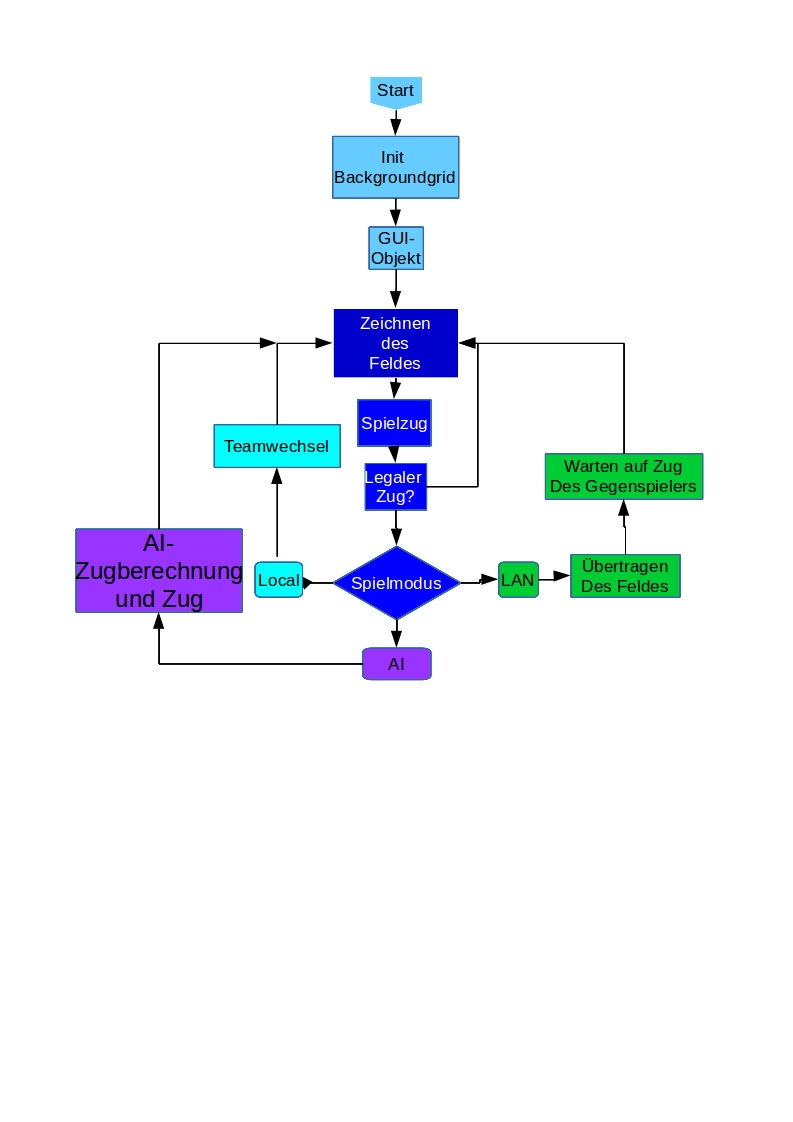
\includegraphics[height=18cm]{graphics/block.jpg}
\cmnt{Blockschaltbild verändern, da init Backgroundgrid und GUI-Objekt vertauscht sind.}

\subsubsection{Initialisierung}
\label{SUBSUBSEC:INIT}

\cmnt{Hier soll erklärt werden wie JavaChess initialisiert wird.}

Als Referenz bzw. Hilfe siehe \ref{SUBSUBSEC:BLOCKSCHALTBILD}.
Zuerst startet das Programm in der Main Methode der Main Klasse. Als nächstes wird das Backgroundgrid Objekt initialisiert und das GUI-Objekt von der GUI-Klasse geladen. \\
Dieses Objekt ladet im Anschluss die Board Gui Klasse, welche ein Canvas ist. In diesem ist eine gewisse Art des Zeichnens möglich. Dadurch wird auch das Schachbrett gezeichnet und in dieser Klasse findet der "Spielfluss" statt. \\ 
Im default Modus startet das Spiel im "Local" game mode, siehe \ref{SUBSEC:LOCAL_MODE}. Hier spielt der Spieler zuerst einen Zug, woraufhin kontrolliert wird ob der Zug legal ist. Da das Spiel im Local-Mode startet, wechselt der Spieler und das Schachbrett wird mit der Aufstellung nach Zug 1 neu gezeichnet.

\subsection{Repräsentation der Figuren:}

Die Figuren werden über eine Zahlenmatrix repräsentiert. Dabei bekommt jede Figur eine individuelle Zahl zugeteilt. \\
Eine solche Zahl besteht aus 3-Ziffer, z.B.: 102. Diese ist der 2. weiße Bauer, die 1. Ziffer gibt dabei an, ob es Team Weiß (1) oder Schwarz (2) ist. Die 2. Ziffer gibt den Figurentyp an, also Bauer, Turm, etc. Die 3.Ziffer gibt an die wievielte Figur es ist. \\
Diese Matrix ist in einem Objekt von der ,,Background-Matrix'' gespeichert. \\
Zu Beginn einer jeden Partie wird einmal die Startaufstellung im ,,Constructor'' der ,,Background-Matrix'' initialisiert:

\begin{center}
	\begin{tabular}{| c | c | c | c | c | c | c | c |}
		\hline
		110 & 120 	& 	130 & 140 	& 150 	& 131 	& 121 	& 	111 \\ \hline
		101 & 102 	& 	103 & 	104 & 	105 & 	106 & 	107 & 	108 \\ \hline
		0	&	0	& 	0	&	0	&	0	&	0	&	0	&	0	\\ \hline
		0	&	0	& 	0	&	0	&	0	&	0	&	0	&	0 	\\ \hline
		0	&	0	& 	0	&	0	&	0	&	0	&	0	&	0 	\\ \hline
		0	&	0	& 	0	&	0	&	0	&	0	&	0	&	0 	\\ \hline
		201 &	202 &	203	&	204	&	205	&	206	&	207	&	208	\\ \hline
		210 & 	220	&	230	&	240	&	250	&	231	&	221	&	211 \\ 
		\hline	
	\end{tabular}
\end{center}

Durch diese Matrix werden in Folge alle Zugberechnungen, KI-Berechnungen, etc. durchgeführt. \\


\subsection{Zugmechanik und Local-Mode}
\label{SUBSEC:LOCAL_MODE}

Sobald das Spiel geladen und initialisiert ist, wird automatisch der ,,Local'' Spielmodus ausgewählt. Dies ist der Hotseat modus, indem man auf einem Device nacheinander spielt. Dieses eigentliche Spiel geschieht in einem Objekt der ,,BoardGui'' Klasse. Die BoardGui Klasse ist ein Canvas Objekt, also ein Objekt auf dem man zum Beispiel zeichnen kann. Diese Funktion wird ausgenutzt, um das Spielfeld zu zeichnen. Wie dies genau geschieht wird in \TODO erläutert.  \\
Nun ist der weiße Spieler an der Reihe. Welches Team an der Reihe ist, wird durch den Boolean ,,team'' bestimmt. Dieser Spielstand wird in einem Objekt der Backgroundgrid Klasse gespeichert. True bedeutet das der weiße Spieler am Zug ist, false das der Schwarze am Zug ist. \\
Der Spieler kann nun die Figur anwählen, die er bewegen möchte, oder die linke Maustaste gedrückt halten und so die Figur über das Brett ,,schweben'' lassen. In dieser Position werden alle möglichen Bewegungen des Spielsteins angezeigt. Hier ist zu erwähnen, dass potentielle Angriffe anders dargestellt werden, wie eine Bewegung. \\
Nun muss der Spieler nur noch das Feld, auf das er ziehen möchte klicken bzw. die Figur darüber absetzen. Der Move algorithmus berechnet nun ob dieser Zug auch möglich ist, falls dieser Zug erlaubt ist wird die Hintergrundmatrix entsprechend umgeschrieben, entsprechend den neuen Positionen der Figuren. \\
Im Local mode wird jetzt das Team gewechselt und die GUI neu gezeichnet, damit die Änderungen in der Matrix sichtbar werden. 

\subsubsection{Die Move Klasse - Funktion}
\label{SUBSUBSEC:MOVE}

Es gibt aber mehrere Möglichkeiten, wie eine Abfrage des erlaubten Zuges entwickelt werden kann. Unser 1.Ansatz bestand darin, dass jede Figur ihren erlaubten Zug selber überprüft. Hierbei muss klar sein, dass wir für jede Figur ein eigenes Objekt, des jeweiligen Klassentypes (z.B.: Bauer) angelegt haben. Für die Zugüberprüfung wird an die Figur die Position übergeben, wohin sie ziehen soll und das momentane Spielfeld. Ein Boolean als Rückgabwert hat dann indiziert, ob dieser Zug legal war. \\
Bevor eine solche Move Abfrage, aber überhaupt durchgeführt werden kann, muss diese auch aufgerufen werden und erkannt werden welcher Spielstein ausgewählt wurde. Dies geschah über eine weitere Move Klasse
Der 1. Ansatz war somit nicht wirklich eine Klasse sondern auf viele Klassenverteilt. Funktioniert hat dies ohne bekannte Bugs, dadurch ist der Code aber stellenweise sehr unübersichtlich geworden. Das Spiel wurde teilweise unperformant und eine AI mit diesem Ansatz zu schreiben ist schlicht unvorstellbar. \\[2ex]
Der 2. Ansatz bestand darin, alle Zugabfragen in einer Klasse zu implementieren. Dazu wurde dem Objekt dieser Klasse, die Koordinaten des zu bewegenden Spielsteines gegeben, wo dieser ist und wohin gezogen werden soll und das Spielfeld. Geprüft wird wieder, ob der Spielzug erlaubt ist. Auch geschieht die Abfrage, welcher Spielstein ausgewählt wurde wieder über eine extrige Klasse.\\ 
Vorteile ergeben sich aus der Übersicht, das Problem mit der Performance hat sich auch weitestegehend gelöst. Das Problem mit der KI ist aber geblieben und nun ist ein weiteres Problem dazugekommen: Wenn man auf eine Figur klickt erscheinen alle Felder, auf die man ziehen kann. Dies ist mit dieser Implementierung der Move Klasse wiederum eine unmöglichkeit zu programmieren.\\[2ex]
Der 3.Ansatz beschäftigt sich mit der Vorschau der möglichen Züge. Man gibt dem Objekt der Move Klasse einfach alles, was bereits im 2. Ansatz übergeben wurde. Nun wird aber ein int[][] aus möglichen Zügen zurückgegeben. Dies funktionierte ohne Probleme. \\
Das einzige was als Problem deklariert werden kann, ist das dadurch das ,,DRY'' (Don´t repeat yourself) Prinzip verletzt wurde. In der Move Klasse ggab es nun einmal die Abfrage, ob der Zug erlaubt ist und einmal die Abfrage welche Züge erlaubt sind. Für die KI ist es von Vorteil, wenn sie alle möglichen Züge eines Spielsteines bekommt. Es sollte aber auch klar sein welcher Spielstein zuvor auf dem Feld stand, was durch diese Methode nur indirekt möglich ist. \\[2ex]
Der 4.Ansatz nimmt sich allen diesen Problemen an, indem den 3. Ansatz ausbaut und eine neue ,,MovePos'' Klasse einführt. Die Move Klasse kann nun als eine Art Box verstanden werden: Man sagt der Move Methode welche Figur man ausgewählt hat und man erhält alle möglichen Züge als MovePos-ArrayList zurück. Der eigentliche Zug muss aber extern durchgeführt werden. \\
Das Objekt der Klasse MovePos, beinhaltet die alte Position des Spielsteins, die neue Position, die ID des Spielsteins, die ID des Feldes auf das gezogen wurde und für die Rochade bzw. den En-Passant noch zwei weitere Informationen zu den Feldern, wo und was darauf war. \\
Dadurch wird für die KI Berechnung, für die Zugüberprüfung und für das Anzeigen aller möglichen Züge die gleiche Basisstruktur der Zugberechnung verwendet. Der Unterschied besteht darin, dass die KI direkt die Zugberechnung aufruft währenddessen die Zugüberprüfung und das Anzeigen der möglichen Züge auf die Methode GetMove zurückgreift (überschreiben das Spielfeld).\\


\subsubsection{Die Move Klasse - Code}
\label{SUBSUBSEC:MOVECODE}
%TODO


Die Move Klasse beinhaltet momentan ca. 1400 Zeilen Code. \\
Die folgende Dokumentation erfolgt als Pseudo Code:

\lstset{language=Java}
\begin{lstlisting}
import...
...
public class Move{
	private ArrayList _HitList;
	private ArrayList _MoveList;
	private ArrayList _LastMoveList;
	private boolean _bSelect;
	private int _iSelect;
	...
	public Move(){
		_bSelect = false;
		...
		das Standardmaessig keine Figur ausgewaeht wurde
		...
	}			
	...
	//Methode fuer Spielerzug bzw. zum anzeigen aller moeglichen Positionen
	public int[][] GetMove(Position und ID von Spielfigur, Objekt von Hintergrundmatrix){
		...
		//Die Differenz zwischen zuvor ausgewählter Figur und jetzt ausgewählten Zug Feld		
		iDif = iPos - _iSelect
		//Wenn die Figur bewegt werden darf
		if(_bSelect && iDif >= 50){
			//ArrayList von der Klasse MovePos
			ArrayList MoveList = getMoveMeeple(Spielfeld,Team, Position Figur)
			for(MovePos MP in MoveList){
				if(MP-Position == Gewaehlte Position){
					...
					Ueberschreiben des alten Feldes mit den neuen Positionen
					Auch fuer alle Spezialzuege
					...		
				}
				
			}
		} else {
			...
			alle moeglichen Zuege
			...
			if(Position ist Figur){
				ArrayList MoveList = getMoveMeeple(Spielfeld,Team,Position Figur)
				for(MovePos MP in MoveList){
					if(Zug auf Leeres Feld){
						_MoveList.add(GezogenesFeld)
					}else{
						_HitList.add(GezogenesFeld)
					}
				}
			}
		}	
		return GeaendertesSpielfeld		
	}
	
	//Herzstueck der Move Klasse - gibt alle moeglichen Zuege zurueck
	public ArrayList getMoveMeeple(Spielfeld, Position von Spielfigur){
		new ArrayList MovePos...MP
		if(Bauer){
			//Zuege
			if(einfacher Zug moeglich){
				MovePos Zug...
				...
				MP.add(Zug) 
				...			
			}
			if(zweifacher Zug moeglich){
				MovePos Zug...
				....
				MP.add(Zug)
				...
			}
			//Schlaege
			if(weisses Team){
				if(Schlag diagonal nach links moeglich){
					MovePos Zug...
					....
					MP.add(Zug)
					...
				}
				if(Schlag diagonal nach rechts moeglich){
					MovePos Zug...
					....
					MP.add(Zug)
					...
				}
			} else {
				if(Schlag diagonal nach links moeglich){
					MovePos Zug...
					....
					MP.add(Zug)
					...
				}
				if(Schlag diagonal nach rechts moeglich){
					MovePos Zug...
					....
					MP.add(Zug)
					...
				}
			}
			//EnPassant
			if(min. 2. Zug){
				...
				letzerZug = getLastMove
				...
				if(wenn feindlicher Bauer danebensteht && ID letzer Zug == id Bauer daneben && Im letzen Zug 2 Felder bewegt worden sind){
					MovePos Zug...
					....
					MP.add(Zug)
					...
				}
			}	
		}else if(Turm){
			for(i=1 bis 7){
				if(Feld in X bzw. Y Richtung Ziehbar bzw. Figur schlagbar && keine Figur dazwischen) {
					MovePos Zug...
					....
					MP.add(Zug)
					...
				}
			}
		
		}else if(Springer){
			if(Feld auf eine von acht Arten ziehbar / schlagbar){
				MovePos Zug...
				....
				MP.add(Zug)
				...
			}
		}else if(Lauefer){
			for(i=1 bis 7){
				if(Feld in eine von vier Richtungen schlagbar/ziehbar){
					MovePos Zug...
					....
					MP.add(Zug)
					...
				}
			}
		}else if(Dame){
			for(i=1 bis 7){
				if(Feld in eine von vier Richtungen schlagbar/ziehbar){
					MovePos Zug...
					....
					MP.add(Zug)
					...
				}
				if(Feld in X bzw. Y Richtung Ziehbar bzw. Figur schlagbar && keine Figur dazwischen) {
					MovePos Zug...
					....
					MP.add(Zug)
					...
				}
			}
		
		}else if(Koenig){
			if(Standard Zuege moeglich){
				MovePos Zug...
				....
				MP.add(Zug)
				...
			}
			if(Feld 4 Felder links vom Koenig leer){
				if(Check Rochade Bedingungen-alle Felder dazwischen leer-kein Feld ist bedroht){
					MovePos Zug...
					....
					MP.add(Zug)
					...
					
				}
			}
			if(Feld 3 Felder rechts vom Koenig leer){
				if(Check Rochade Bedingungen-alle Felder dazwischen leer-kein Feld ist bedroht){
					MovePos Zug...
					....
					MP.add(Zug)
					...
				}
			}
		
		}
		
		return MP;
	}
	
	...
	Methode Bauerntausch
	...
	getSchach //ueberprueft ob Koenig im Schach ist (=vl. illegaler Zug)-via Schachmatt Methode
	getSchach2 //ueberprueft ob Koenig im Schach ist (Warnung an Spieler)-via Schachmatt Methode
	...
	getter und setter Methoden fuer Private Variablen
}
\end{lstlisting}
\lstset{language=German}

\subsection{Schach und Schachmatt Abfrage:}
\label{SUBSEC:checkmate}

Die Schachmatt Abfrage teilt sich in drei Methoden innerhalb der Backgroundgrid Klasse auf:
\begin{itemize}
	\item{\nameref{SUBSUBSEC:check}}
	\item{\nameref{SUBSUBSEC:checkmate}}
	\item{\nameref{SUBSUBSEC:checkking}}
\end{itemize}



\subsubsection{Schach}
\label{SUBSUBSEC:check}

Die Schachmethode kann auf JEDE Figur angewendet werden und gibt TRUE zurück, wenn diese von einer anderen Figur angegriffen werden kann. Logisch gesehen gibt sie FALSE zurück, wenn die Figur nicht angegriffen werden kann. \\
Im Prinzip werden alle Figuren aufgerufen und überprüft ob diese die ,,ausgewählte'' Figur angreifen können. \\
Pseudo Code:

\lstset{language=Java}
\begin{lstlisting}
private boolean Schach(Spielfeld, Lokation der Spielfigur auf die Schach angewendet werden soll){
	for(alle Figuren){
		if(Figur ist Bauer und kann Spielfigur angreifen){
			return true;		
		} else if(Figur ist Turm und kann Spielfigur angreifen){
			return true;
		} else if(Figur ist Springer und kann Spielfigur angreifen){
			return true;
		} else if(Figur ist Laeufer und kann Spielfigur angreifen){
			return true;
		} else if(Figur ist Dame und kann Spielfigur angreifen){
			return true;
		} else if(Figur ist Koenig und kann Spielfigur angreifen){
			return true;
		}
		
	}
	
	return false;	
}
\end{lstlisting}
\lstset{language=German}

\subsubsection{Schachmatt}
\label{SUBSUBSEC:checkmate}

Die Schachmatt Methode kann nur auf den Koenig angewendet werden. Diese überprüft nacheinander alle Bedingungen, ob der Koenig wirklich Schachmatt ist. Anfangs wird überprüft ob er dem Angreifer ausweichen kann bzw. schlagen kann. Falls dies nicht möglich ist wird überprüft ob der Angreifer selbst geschlagen werden kann. \\
Anschließend wird überprüft, ob es möglich ist, zwischen den Angreifer und den König mit irgendeiner Figur zu springen. \\
Pseudo Code:

\lstset{language=Java}
\begin{lstlisting}
private boolean Schachmatt(Spielfeld, ID und Postion des Koenigs, Backgroundgrid Objekt){
	for(Positionen wo Koenig hinziehen kann){
		if(Position nicht bedroht){
			return false;
		}
	}
	
	if(Schach Methoden auf Angreifer anwenden == TRUE){
		return false;
	}
	
	for(alle moeglichen Zuege des Angreifers){
		for(alle Figuren des anderen Teams){
			for(alle Zuege der Figur)7
				if(Zug moeglich && dadurch Koenig nicht mehr im Schach){
					return false;
				}
			}			
		}
	}
}
\end{lstlisting}
\lstset{language=German}


\subsubsection{Schachking}
\label{SUBSUBSEC:checkking}

Schachking wird immer am Ende eines Zuges aufgerufen und überprüft ob ein Team Schachmatt ist. Falls dieser nicht Schach oder Schachmatt ist, wird nachgesehen ob eine Patt Situation vorrherrscht. Dies geschieht in der Draw Methode. \\
Falls ein Team Schach ist wird nachgesehen ob dieser auch Schachmatt ist. \\
Pseudo Code:

\lstset{language=Java}
\begin{lstlisting}
public boolean Schacking(team,Spielfeld,auf welche Figur/Position die Abfrage gemacht werden soll, Schachmatt/Schach, simulierter Koenig){
	ID = ID des Koenigs
	
	Schach Abfrage auf ID
	
	if(wenn Schach nicht zutrifft und Schachmatt ausgefuehrt werden soll){
		Patt Situation soll ermittelt werden
	}
	if(wenn Schach zutrifft und Schachmatt ausgefuehrt werden soll){
		Schachmattabfrage
		if(Schachmatt trifft zu und weisses Team){
			weisses Team verliert
		}	
		if(Schachmatt trifft zu und schwarzes Team){
			schwarzes Team verliert
		}
	}
}
\end{lstlisting}
\lstset{language=German}

\subsection{LAN-Mode}

%TODO
%@Huber das hier ist was für dich 

\subsection{AI-Mode}

Wie funktioniert die AI (Artificial Intelligence) des Schachspiels? \\
Für die Beantwortung dieser Frage werden folgende Kapitel behandelt:

\begin{itemize}
	\item{\nameref{SUBSUBSEC:GenAI}}
	\item{\nameref{SUBSUBSEC:OurAI}}
	\item{\nameref{SUBSUBSEC:MinMax}}
	\item{\nameref{SUBSUBSEC:AICODE}}
\end{itemize}



\subsubsection{Prinzipielle Moeglichkeiten einer AI}
\label{SUBSUBSEC:GenAI}

Der Terminus "AI" wird sehr oft verwendet, jedoch gibt es Unterschiede zwischen den AIs die größer nicht sein könnten. So gibt es zum Beispiel Künstliche Intelligenzen die durch Machine-Learning-Algorithmen basieren und andere, einfachere, denen ein Min-Max Prinzip zu Grunde liegt. \\
Das Min-Max Prinzip lässt sich aber nur bei Spielen mit perfekter Information anwenden, wie Schach eines ist. Ein Spiel mit perfekter Information bedeutet, dass jeder Spieler alles weiß, so haben im Schach immer beide Spieler das gesamte Spielfeld im Blick. \\[2ex]
Durch diese Art des Spiels können die theoretisch besten Züge ermittelt werden, um den besten möglichen Zug zu ziehen. Dazu muss der Algorithmus alle möglichen Spielzüge analysieren, bewerten und vergleichen um zu einem Zug zu machen. Dies ist ein sehr hoher Rechenaufwand, dafür einfacher zu implementieren. Diese Art der AI haben wir verwendet, siehe \ref{SUBSUBSEC:OurAI}. \\[3ex]
Die andere Möglichkeit ist ein Machine-Learning-Algorithmus. Dieser versucht ein biologisches Gehirn nachzubauen, indem es ein Künstliches-Neurales-Netzwerk bildet. Diese Neuronen werden dahingehend trainiert, dass die AI aus einem gegebenen Satz Daten und/bzw. mit Hilfe einer Lernfunktion Rückschlüsse auf mögliche zukünftige Ereignisse schließt. Mathematisch gesehen basiert diese Art der KI auf der Wahrscheinlichkeitsrechnung.  \\
Wichtig ist noch anzumerken, dass diese Art der KI selber lernen kann wie sie besser wird. Als Beispiel nehmen wir Schach, die KI spielt über längere Zeit gegen sich selber und muss um sich zu verbessern nicht unbedingt gegen andere Spieler, sowohl menschlich als auch maschinell antreten. \\
Maschinelles Lernen ist ein sehr umfangreiches Thema, womit hier nur noch gesagt sei, dass maschinelles Lernen in letzter Zeit einige Durchbrüche erlebt hat. Um noch ein konkretes Beispiel zu nennen: Im Dezember 2017 gewann der von Google entwickelte Algorithmus AlphaZero gegen die Chess-Engine ,,Stockfish 8''. AlphaZero basiert auf maschinellen Lernen und Stockfish 8 auf der Vorausberechnung aller möglichen Züge. \\[2ex]
Wieso wurde die AI nicht im maschinellen Lernen verfahren entwickelt? \\
Dies hätte den Rahmen der Diplomarbeit gesprengt und wäre für sich allein genommen eine eigene Diplomarbeit.

\subsubsection{Verwendete Schach-AI-Funktion}
\label{SUBSUBSEC:OurAI}

Wie vorher schon beschrieben verwendet die Java-Chess-AI eine Abwandlung des Min-Max Algorithmus. Dieser wird ,,alphaBeta'' Algorithmus genannt. \\
Prinzipiell sucht der Algorithmus nach dem besten Spielzug. Um dies tun zu können, benötigt es einen Algorithmus welcher alle möglichen Spielzüge bis zu einer gewissen Tiefe durchsucht und den besten Spielzug in Folge herausschreibt. \\ 
Hierfür muss geklärt werden, welcher Spieler gerade die Oberhand hat. Im entwickelten Algorithmus besteht die fundamentale ,,Board-Evaluation'' aus der Materiellen Balance. Also welcher Spieler hat mehr und bessere Figuren. Anschließend werden noch  ,,Bauernformationen'', also wenn die Bauern sich gegenseitig decken und sogenannte ,,Piece Square Tables'' in die Kalkulation mit eingerechnet. Piece Square Tables geben an, wo die Figuren statistisch gesehen am besten stehen. Zum Beispiel stehen Türme lieber in der Mitte, als am Rand. Dadurch haben sie mehr Bewegungsfreiheit, was im Schachspiel eine der wichtigsten Strategien zum Sieg ist. Hierbei muss angemerkt werden, dass die Piece Square Tables von SchachmeisternInnen erstellt wurden, welche der Öffentlichkeit zugänglich gemacht worden sind. \\[2ex]
Das Durchsuchen der möglichen Spielzüge läuft folgendermaßen ab: Es wird zuerst festgelegt bis zu welcher Tiefe (z.B.: 5) gesucht werden soll. Anschließend wird der 1. mögliche Zug getätigt. Anschließend ruft sich die Methode selbst rekursiv auf, wobei die Tiefe erhöht und das Team gewechselt wird und tätigt wiederum den 1. möglichen Zug. Dies geschieht solange bis die gewünschte Tiefe (5) erreicht ist, bei welcher die ,,Board-Evaluation'' durchgeführt wird. Dieser Wert wird zwischengespeichert und der zuletzt getätigte Zug wird rückgängig gemacht. \\
Nun befindet sich der Algorithmus wieder in der Tiefe 4, in welcher der 2.mögliche Zug getätigt wird. Falls dieser Zug besser ist als der vorherige, überschreibt dieser den zwischengespeicherten 1. Zug. Falls nicht, wird er von nun an nicht länger berücksichtigt. \\
Dies geschieht nun solange, bis alle relevanten Züge durchsucht wurden, welche nicht relevant sind wird in \ref{SUBSUBSEC:AICODE} behandelt. \\
Sobald der beste Zug ermittelt wurde, folgt die übliche Schachmatt-Abfrage und das Überschreiben des Schachfeldes mit den neuen Positionen. Anschließend ist wie in \ref{SUBSUBSEC:BLOCKSCHALTBILD} gezeigt, wieder der Spieler an der Reihe. \\[2ex]
Eines der größten Probleme des Algorithmus ist die Performance. Dazu ein simples Gedankenexperiment: Beim 1. Spielzug sind 20 mögliche Züge des weißen Spielers möglich und ebensoviele beim darauffolgenden Zug des schwarzen Spielers. Daraus resultiert aus den beiden Spielzügen \(20 \cdot 20 = 400\) verschiedene Stellungen. \\
Gemittelt gibt es im Schach 28 mögliche Züge pro Spielzug. Nach 5 Zügen ergeben sich daraus schon 3.200.000 mögliche Stellungen, nach 6 wären es 64.000.000. Um zu einer Entscheidung zu kommen muss der Computer alle diese Züge analysieren und bewerten. Dies benötigt Rechenleistung, weshalb ein solcher Schachalgorithmus sehr abhängig von der verwendeten Hardware ist. \\
Im weiteren Sinne ist dies der Grund warum solche künstlichen Intelligenzen gegen Künstliche-Neuronale-Netzwerke verlieren (siehe \ref{SUBSUBSEC:GenAI}). Die Min-Max Algorithmen können nicht ausreichend optimiert werden bzw. moderne Hardware besitzt einfach nicht genügend Rechenleistung um diesen Wettlauf standzuhalten. \\

\subsubsection{Der MinMax-Algorithmus:}
\label{SUBSUBSEC:MinMax}

In den Kapiteln \ref{SUBSUBSEC:GenAI} und \ref{SUBSUBSEC:OurAI} wurde erwähnt, dass die JavaChess AI nach dem Min-Max Prinzip funktioniert, nur was ist dieses Prinzip?

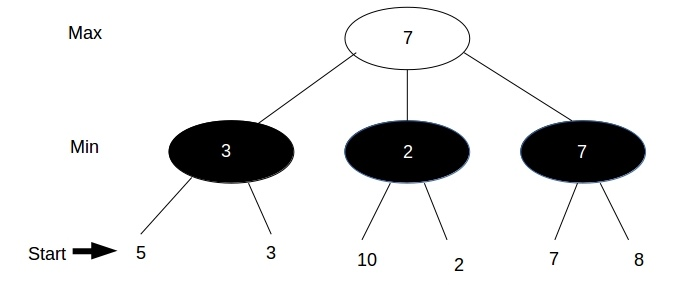
\includegraphics[width=16cm]{graphics/MinMax.jpg}

MinMax ist nichts anderes, als das Erhalten des bestmöglichen Ergebnisses für einen Spieler, wenn die Züge des Gegenspielers miteingerechnet werden. In diesem Beispiel haben wir zwei Teams, Weiß und Schwarz. Diese sind durch die weißen Blasen erkenntlich. Weiters gilt für ein kompetitives Spiel wie Schach, dass das weiße Team immer ihr bestes Ergebnis herausholen möchte und das Schwarze auch ihres. Die Zahlen repräsentieren die Günstigkeit der Stellung für das weiße Team, wobei 10 die best mögliche Stellung ist und 1 die schlechteste. Für das schwarze Team ist dies umgekehrt, für sie ist 10 das schlechteste Ergebnis und 1 das Beste. \\
Somit wird das schwarze Team immer das kleinere Ergebnis nehmen, quasi das MINIMUM herausholen (=Min) und die Weißen immer das höchstmögliche, also das MAXIMUM (=Max). Daher auch der Name, MinMax. \\
Zurück zum Beispiel: Schwarz kann einmal wählen zwischen den Zahlen 5 \& 3, zwischen 10 \& 2 und zwischen 7 \& 8. Da die Schwarzen immer die niedrigere Zahl nehmen, kann die niedrigere Zahl in den schwarzen Bubble geschrieben werden (3, 2 \& 7). \\
Somit muss sich der weiße Spieler nur noch zwischen 3 Zahlen entscheiden, bei denen er die höchste nimmt, also 7. Dies ist das best mögliche Ergebnis für das weiße Team.

\subsubsection{Code}
\label{SUBSUBSEC:AICODE}

Die theoretischen Grundlagen zum Verständnis des Algorithmus sollten nun geklärt sein.\\
Die KI besteht aus zwei Klassen, AI und AILogic. AI wird als neuer Thread ausgeführt. \\
Der nachfolgende Code zur AI erfolgt als Pseudo-Code Dokumentation.


Klasse AI:

\lstset{language=Java}
\begin{lstlisting}
	public class AI extends Thread{
		public void run(){
			AIL = initialisiere AILogic()
			AIL.alphaBeta()
			//Besten Zug bekommen
			Move = AIL.getMove()
			
			Hintergrundmatrix mit Move veraendern.
		}
	}	
\end{lstlisting}

Klasse AI-Logic:
\lstset{language=Java}
\begin{lstlisting}
	public class AILogic{
	
		private MaximaleTiefe
		//wird benoetigt um die maximale Tiefe festzulegen und um den Logarithmus zu verbessern
		public float alphaBeta(tiefe, Hintergrundmatrix, Team){
			MaximaleTiefe = tiefe
			alpha = 10000
			beta = -10000
			for(i<tiefe){
				//Fuer den AlphaBeta algorithmus
				beta = alphaBetaHelper(starte bei Tiefe 0, BackgroundMatrix, alpha,beta)
			}
			
		}	
	
		//der AlphaBeta Algorithmus - zur Zugevaluation 
		public float alphaBetaHelper(tiefe, Hintergrundmatrix, Team, alpha, beta){
			Sum = boardEvaluation
			
			if(Sum bedeutet das feindlicher Koenig geschlagen wird){
				return 20000
			}
			
			if(tiefe >= MaximaleTiefe){
				return Sum
			}
			
			for(X und Y Positionen des Spielfeldes){
				if(Spielfigur an Position){
					Zuege = AlleMoeglichenZuegeDerSpielfigur
					for(alle Moeglichen Zuege der Figur){
						A = Zug						
						Den Zug auf das Spielfeld uebertragen
						
						Sum1 = -alphaBetaHelper(tiefe+1, BackgroundGrid, Teamwechsel, -alpha, -beta)
						
						Den Zug rueckgaengig machen		
						
						if(Sum1 >= beta){
							beta = Sum1	
							if(Sum1 >= alpha){
								return alpha
							}			
							if(tiefe == 0){
								ZuListeGuterZuegeHinzufuegen(A)						
							}
						}	
						
					}
				}
				
			}
		return beta			
		}
		
		public float boardEvaluation(Backgroundgrid, Team){
			//Fuer die Material Balance
			
			for(X und Y Positionen des Spielfeldes){
				if(Bauer weisses Team){
					100 Punkte zum weissen Team dazu zaehlen
					Punkte entsprechend der Bauerntabelle hinzuzaehlen
					Punkte nach Bauerntabelle hinzuzaehlen
				} else if(Turm weisses Team){
					500 Punkte zum weissen Team dazu zaehlen
					Punkte entsprechend der Turmtabelle hinzuzaehlen
				} else if(Springer weisses Team){
					325 Punkte zum weissen Team dazu zaehlen
					Punkte entsprechend der Springertabelle hinzuzaehlen
				} else if(Lauefer weisses Team){
					300 Punkte zum weissen Team dazu zaehlen
					Punkte entsprechend der Lauefertabelle hinzuzaehlen
				} else if(Dame weisses Team){
					900 Punkte zum weissen Team dazu zaehlen
					Punkte entsprechend der Damentabelle hinzuzaehlen
				} else if(Koenig weisses Team){
					10000 Punkte zum weissen Team dazu zaehlen
					Punkte entsprechend der Koenigtabelle hinzuzaehlen
				}
				
				if(Bauer schwarzes Team){
					100 Punkte zum schwarzen Team dazu zaehlen
					Punkte entsprechend der Bauerntabelle hinzuzaehlen
					Punkte nach Bauerntabelle hinzuzaehlen
				} else if(Turm schwarzes Team){
					500 Punkte zum schwarzen Team dazu zaehlen
					Punkte entsprechend der Turmtabelle hinzuzaehlen
				} else if(Springer schwarzes Team){
					325 Punkte zum schwarzen Team dazu zaehlen
					Punkte entsprechend der Springertabelle hinzuzaehlen
				} else if(Lauefer schwarzes Team){
					300 Punkte zum schwarzen Team dazu zaehlen
					Punkte entsprechend der Lauefertabelle hinzuzaehlen
				} else if(Dame schwarzes Team){
					900 Punkte zum schwarzen Team dazu zaehlen
					Punkte entsprechend der Damentabelle hinzuzaehlen
				} else if(Koenig schwarzes Team){
					10000 Punkte zum schwarzen Team dazu zaehlen
					Punkte entsprechend der Koenigtabelle hinzuzaehlen
				}
			}
		}
		
		...Tabellen fuer Bauern, Lauefer,...		
		
	}	
\end{lstlisting}
\lstset{language=German}

%=================================================================================
\clearpage\vfill\newpage{}
%=================================================================================
\section{ChessPI}
\label{SEC:chesspi}

ChessPI ist die Implementierung von JavaChess auf dem Raspberry PI. \\
Wir haben uns zur Aufgabe gestellt das Schachprogramm auch auf einem Mikro-Computer zum funktionieren zu bekommen. An dem RaspberryPI wird ein Touchscreen angeschlossen, mit welchem der User interagieren kann. Weiters soll für den RaspberryPI mit angeschlossenen Touchscreen ein Gehäüse designt und eine Akkusteuerung entworfen werden. 
Die Probleme die dabei auftreten könne sind unzählig, die hauptprobleme können aber determiniert werden:
\begin{itemize}
	\item{Der RaspberryPI besitzt zu wenig Rechenleistung}
	\item{Die verfügbaren Java Versionen beinhalten nicht die von uns verwendeten Packages}
	\item{Das Spiel ist nicht über einen Touchscreen spielbar}
\end{itemize}

\subsection{RaspberryPI}

Der Raspberry PI ist ein vollwertiger Computer, welcher mit einem Linux/GNU OS läuft. Am häufigsten wird die Distribution Raspbian verwendet. \\
Die von uns verwendete Version ist der Raspberry PI 3 model B. Dieser verfügt über eine Quad Core 1.2 GHz Broadcom BCM2837 CPU, 1 GB an RAM. Dies ist eine deutliche Steigerung gegenüber den vorherigen Modellen, womit das Problem notwendige Leistung zumindest leicht gelöst wird. \\

\subsection{Touchscreen}

Als Touchscreen wird das Ofizielle 7" Touchscreen Display verwendet. Dies hat eine Auflösung von 800x480 Pixel. \\
Zusätzlich zum Display gibt es auch eine Adapterplatine, mit der der Touchscreen versorgt wird. \\
Halterungen für die Adapterplatine und den Raspberry PI gibt es auf der Rückseite des Touchscreens.

\subsection{Implementierung von JavaChess}

Alle benötigten Schritte beziehen sich lediglich auf die Software Implementation, nicht auf die Hardware Implementation (Powerbank, Gehäuse). \\[1ex]

\textbf{Vorbereitung:} \\[2ex]
Es wird ein RaspberryPI 3, eine mikro SD-Karte mit Raspbian, eine Stromversorgung bzw. eine Powerbank mit einem maximalen Strom von 2.5 A, der 7" Touchscreen, die Adapterplatine, eine Internetverbindung idealerweise über ein LAN-Kabel und eine USB-Tastatur benötigt. \\

\begin{enumerate}
	\item{Die SD Karte mit Raspbian wird in den Raspberry PI gegeben}
	\item{Die Adapterplatine und der Raspberry PI wird auf den Touchscreen geschraubt}
	\item{Die Stromversorgung für den Display (VCC \& GND Pin- rotes und blaues Kabel) wird sichergestellt. Das Flachbandkabel / Datenkabel wird zwischen Raspberry PI und Adapterplatine angebracht.}
	\item{Der Raspberry Pi wird an die Stromversorgung angeschlossen, dadurch sollte dieser nun booten und den Display automatisch erkennen.}
	\item{Sobald Raspbian gebootet hat, wird das LAN-Kabel angeschlossen.}
	\item{Nun sollten folgende Befehle in der BASH ausgeführt werden:}
	\begin{enumerate}
		\item{sudo apt-get update}
		\item{sudo apt-get upgrade}
		\item{sudo apt-get install oracle-java8-jdk}
		\item{reboot}
	\end{enumerate}
	\item{Nun wurde Java installiert. Es muss noch JavaFX ,,dazuinstalliert'' werden, da dies nicht in der Java-Embedded-JDK Serie enthalten ist.}
	\item{Es muss OpenJFX gedownloaded werden. URL: https://chriswhocodes.com/}
	\item{Hier die Version für den Raspberry PI downloaden (ARMv6)}
	\item{Die gedownloadete OpenJFX Zip muss im Installationsverzeichnis ovn Java-JDK8 ,,unzipped'' werden.}
	\item{In Commandline wird nun folgender Befehl ausgeführt: unzip openjfx-sdk-overlay-linux-arm6hf.zip -d /<installations-verzeichnis-von-Java (z.B.: /home/pi/jdk1.8.0_92)>}
	\item{Nun wird das aktuelle Schachspiel gedownloaded (die Jar), URL: https://github.com/alexl4123/diplomarbeit/releases}
	\item{Das Schachspiel wird in das Verzeichnis der Wahl abgelegt.}
	\item{Nun kann das Schachspiel gestartet werden, dazu muss der Touchscreen aber noch konfiguriert werden, da sonst ein ,,interessanter'' Offset geschieht.}
	\item{Dazu muss zuerst der Touchscreen identifiziert werden: cat /sys/class/input/event1/uevent}
	\item{Bei dem versuchs Raspberry PI war dieses Input Device: 0/0/0/0}
	\item{Um das Schachspiel bequem zu öffnen wird empfohlen ein BASH-Skript zu erstellen:}
	\item{\# /bin/bash \\
	java -Dmonocle.input.0/0/0/0.minX=0 -Dmonocle.input.0/0/0/0.minY=0 -Dmonocle.input.0/0/0/0.maxX=800 -Dmonocle.input.0/0/0/0.maxY=500 -jar chess.jar}
	\item{Nun das Skript öffnen: sudo ./<skript>}
	\item{Das Schachspiel sollte sich nun öffnen.}
\end{enumerate}
	

%TODO

%=================================================================================
\clearpage\vfill\newpage{}
%=================================================================================
\section{Akkusteuerung}
\label{SEC:death}


%=================================================================================
\clearpage\vfill\newpage{}
%=================================================================================
\section{Gehäuse}
\label{SEC:case}


%=================================================================================
\clearpage\vfill\newpage{}
%=================================================================================
\section{Android}
\label{SEC:android}


%=================================================================================
\clearpage\vfill\newpage{}
%=================================================================================
\section{\sc Fertigungsdokumentation}
	{\yhbu
	Die Fertigungsdokumentation ist als optionaler Dokumentationsteil zu sehen und
	wird mit der Betreuerin bzw. Betreuer besprochen, ob dieser Teil der Dokumentation
	notwendig ist. Gedacht ist die Fertigungsdokumentation speziell für aufwändige
	Schaltungen, bei denen es notwendig erscheint, einen Verkabelungsplan, spezielle
	Anleitungen für das Einlöten der Bauteile usw. auszuarbeiten.
	}
\section{\sc Benutzerdokumentation}
	{\yhbu
	Hinweis: Die Benutzerdokumentation beschreibt das System aus der Sicht des
	Benutzers. Ein beliebiger Benutzer sollte in die Lage versetzt werden, das System
	zu verwenden (Bedienungsanleitung, technische Dokumentation).
	}
 \subsection{Installationsanleitung}
	{\yhbu
	Schritt-für-Schritt-Anleitung, wie das System vom Benutzer erstmalig in Betrieb
	genommen werden kann. Weiters eine Anleitung, wie die Software des Systems mit
	Hilfe der Entwicklungswerkzeuge neu erstellt werden kann.
	}
 \subsection{Anwendungsbeispiele}
	{\yhbu
	Beschreibung typischer Aufgaben, die der Benutzer mit dem System durchführen
	kann (Schritt-für-Schritt-Anleitungen).
	}
 \subsection{Referenzhandbuch}
	{\yhbu
	Beschreibung der einzelnen Bedienungselemente (Frontplatten, Dialoge...).
	}
 \subsection{Fehlermeldungen und Hinweise auf Fehlerursachen}
	{\yhbu
	Alle Fehlermeldungen, die das System dem Benutzer ausgeben kann, mit
	Beschreibung der Ursache und Vorschlägen zur Lösung des Problems.
	}









%=================================================================================
\clearpage\vfill\newpage{}
%=================================================================================
\renewcommand{\thesection}{\Roman{section}\;}
%\renewcommand{\labelsection}{(\roman{section})}
\setcounter{section}{0}
%\section{\sc \;}\hfill\\[-24mm]
	%Abbildung 2: Zeitplanung Projekt	8
\section{\sc Abbildungsverzeichnis}\noindent%
	\\ Abbildung 1: Datenübertragungsrate SDRAM
	(Quelle: Einfache IT-Systeme, 2009, S.56) \dotfill vi
	\\ Abbildung 2: Projektzeitplan \dotfill VI
	\\[4mm]{\korr $\to$ \LaTeX\, erstellt mit {\em'\tbs{}listoffigures'}
	Abbildungsverzeichnisse vollautomatisch}


%\section{\sc \;}\hfill\\[-23mm]
	%Tabelle 1: Arbeitsaufstellung	9
\section{\sc Tabellenverzeichnis}\noindent%
	\\ Tabelle 1: Arbeitsaufstellung \dotfill VII
	\\[4mm]{\korr $\to$ \LaTeX\, erstellt mit {\em'\tbs{}listoftables'}
	Abbildungsverzeichnisse vollautomatisch}










%=================================================================================
\clearpage\vfill\newpage{}
%=================================================================================
\renewcommand{\thesection}{\Roman{section}\;}
\setcounter{section}{2}
%\vspace*{-8mm}
\section{\sc Literaturverzeichnis}
	{\yhbu
	Beispiele:
	\\[0mm]{\fontsize{10pt}{10pt}\selectfont
	(Übernommen aus dem Leitfaden des BMBF Reife- und Diplomprüfungen März 2014)
	\\[0mm]
	\begin{description*}
	\item[1. Werke eines Autors] Nachname, Vorname: Titel. Untertitel. -
		Verlagsort: Verlag, Jahr. Nachname,
		Vorname: Titel. Untertitel. Auflage - Verlagsort: Verlag, Jahr.
		\\[1mm]Beispiele:
		\\Sandgruber, Roman: Bittersüße Genüsse. Kulturgeschichte der Genußmittel. – Wien:
		Böhlau, 1986. Messmer, Hans-Peter: PC-Hardwarebuch. Aufbau, Funktionsweise,
		Programmierung. Ein Handbuch nicht nur für Profis. 2. Aufl. - Bonn: Addison-Wesley,
		1993.
		\vspace*{2mm}
	\item[2. Werke mehrerer Autoren] Nachname, Vorname; Nachname, Vorname; Nachname, Vorname: Titel.
		Untertitel. Auflage - Verlagsort: Verlag, Jahr.
		\\[1mm]Beispiel:
		\\Bauer, Leonhard; Matis, Herbert: Geburt der Neuzeit. Vom Feudalsystem zur
		Marktgesellschaft. - Mün- chen: Deutscher Taschenbuch Verlag, 1988.
		\vspace*{2mm}
	\item[3. Sammelwerke, Anthologien, CD-ROM mit Herausgeber] Nachname, Vorname (Herausgeber):
		Titel. Untertitel. Auflage - Verlagsort: Verlag, Jahr. Nachname, Vorname: Titel.
		Untertitel. In: Nachname, Vorname (Herausgeber): Titel. Untertitel. Auflage -
		Verlagsort: Verlag, Jahr.
		\\[1mm]Beispiele:
		\\Popp, Georg (Hg.): Die Großen der Welt. Von Echnaton bis Gutenberg. 3. Aufl. -
		Würzburg: Arena, 1979. Killik, John R.: Die industrielle Revolution in den Vereinigten
		Staaten. In: Adams, Willi Paul (Hg.): Die Vereinigten Staaten von Amerika. Fischer
		Weltgeschichte Bd. 30. - Frankfurt am Main: Fischer Taschenbuch Verlag, 1977. Killy,
		Walther (Hg.): Literatur Lexikon. Autoren u. Werke deutscher Sprache. – München:
		Bertelsmann, 1999. (Digitale Bibliothek, 2)
		\vspace*{2mm}
	\item[4. Mehrbändige Werke] Nachname, Vorname: Titel. Bd. 3 - Verlagsort: Verlag, Jahr.
		\\[1mm]Beispiel:
		\\Zenk, Andreas: Leitfaden für Novell NetWare. Grundlagen und Installation. Bd. 1 - Bonn:
		Addison Wesley, 1990.
		\vspace*{2mm}
	\item[5. Beiträge in Fachzeitschriften, Zeitungen] Nachname, Vorname des Autors des bearbeiteten
		Artikels: Titel des Artikels. In: Titel der Zeitschrift, Heftnummer, Jahrgang, Seite
		(eventuell: Verlagsort, Verlag).
		\\[1mm]Beispiel:
		\\Beck, Josef: Vorbild Gehirn. Neuronale Netze in der Anwendung. In: Chip, Nr. 7, 1993,
		Seite 26. - Würzburg: Vogel Verlag.
		\vspace*{2mm}
	\item[6. CD-ROM-Lexika]\hfill
		\\[1mm]Beispiel:
		\\Encarta 2000 - Microsoft 1999.
		\vspace*{2mm}
	\item[7. Internet] Nachname, Vorname des Autors: Titel. Online in Internet: URL: www-Adresse, Datum.
		(Autor und Titel wenn vorhanden, Online in Internet: URL: www-Adresse, Datum auf
		jeden Fall)
		\\[1mm]Beispiel:
		\\Ben Salah, Soia: Religiöser Fundamentalismus in Algerien. Online im Internet:
		URL: >>http:/\slash{}www.hausarbeiten.de\slash{}cgi-bin\slash{}superRD.pl<<,
		22.11.2000. Der Weg zur Doppelmonarchie.
		Online in Internet: URL:
		http:/\slash{}www.parlinkom.gv.at\slash{}pd\slash{}doep\slash{}d-k1-2.htm,
		22.11.2000.
		\vspace*{2mm}
	\item[8. Firmenbroschüren, CD-ROM] Werden Inhalte von Firmenunterlagen verwendet,
		dann ist ebenfalls die Quelle anzugeben.
		\\[1mm]Beispiel:
		\\Digitale Turbinenregler. Broschüre der Firma VOITH-HYDRO GmbH, 2012.
		\vspace*{2mm}
	\item[9. Abbildungen, Pläne] Werden Abbildungen aus einer fremden Quelle
		[z.B. Download, Scannen) in die Diplomarbeit eingefügt,
		so ist unmittelbar darunter die Quelle anzugeben.
		\\[1mm]Beispiel:
		\\Abb. 1: Digitaler Turbinenregler [ANDRITZ HYDRO]
		\vspace*{2mm}
	\item[10. Persönliche Mitteilungen]\hfill
		\\[1mm]Beispiel:
		\\Persönliche Mitteilung durch: König, Manfred:
		Kössler GmbH Turbinenbau am 8. März 2013.
	\end{description*}
	}}%yhbu













%=================================================================================
\clearpage\vfill\newpage{}
%=================================================================================
\appendix
\part*{\sc Anhang}
\renewcommand{\thesection}{\arabic{section}\;}
\setcounter{section}{5}
\section{\sc Pflichtenheft}
	{\yhbu
	Zur Umsetzung des Projektzieles werden messbare Kriterien formuliert.
	}
 \subsection{Funktionale Anforderungen}
	{\yhbu
	Die Anforderungen müssen detailliert beschrieben werden,
	sie müssen mess- und überprüfbar sein
	(nicht: \dq{}Antwort so schnell wie möglich\dq{}, sondern: \dq{}Antwort in 0.5s\dq{}).
	\\[1mm]
	Sie definieren das Systemverhalten
	(z. B. Erfassen und Interpretieren von Sensorwerten;
	Suchen von Datenbankeinträgen\ldots).
	Die Interaktionen (Mensch-Maschine, Maschine-Maschine)
	sollen auch graphisch dargestellt werden.
	}

 \subsection{Schnittstellen}
	{\yhbu
	Technische Eigenschaften des Systems nach {\em außen}
	(Hardware- und\slash{}oder Softwareschnittstellen).
	Hier wird nur der Verweis auf verwendete Schnittstellen gegeben,
	aber nicht die Definition oder Erklärung
	(außer bei selbst definierten Schnittstellen).
	}

 \subsection{Abnahmekriterien}
	{\yhbu
	Objektive Kriterien,
	mit denen die Vollständigkeit und Korrektheit
	der fertigen Lösung geprüft werden kann
	(z.B.: Bei einem Signalgenerator wird das Ausgangssignal
	in einem definierten Frequenzbereich mit einem Oszilloskop überprüft).
	\\[1mm]
	Die Prototypen der einzelnen Iterationen
	(im Management ist Iteration eine Vorgehensweise,
	um mit den Ungewissheiten und Überraschungen in komplexen Situationen umzugehen)
	sind zu spezifizieren.
	Die Funktionalität der Prototypen muss durch quantifizierbare Ergebnisse überprüfbar sein.
	Die Spezifikation des Prototypen der nächsten Iteration
	ist bei Präsentation einer Iteration vorzustellen.
	Eine Iteration wird mit der Präsentation des Prototypen abgeschlossen (Meilenstein).
	}

 \subsection{Dokumentationsanforderungen}
	{\yhbu
	Anforderungen, die über das Dokument
	\dq{}Gesamtdokumentation\_Vorlage.doc\dq{} hinausgehen
	(z.B.: Online-Hilfe, Dokumentation in Englisch\ldots).
	}

 \subsection{Qualitätsstandards}
	{\yhbu
	Die im Projekt verwendeten Qualitätsstandards und einzuhaltende Normen
	werden festgelegt,
	z.B. hausinterne oder industrielle Printfertigung, verwendete Normen\ldots
	}

 \subsection{Abwicklungsprozess}{\yhbu
	Für die Projektabwicklung an der
	Abteilung für Elektronik und Technische Informatik der HTL-Anichstrasse
	gelten folgende Phasen:
	\\[4mm]\hspace*{-3mm}
	\begin{tabular}{p{50mm} l}
	Startphase Phase \#1
			&(Sommersemester 4. Klasse):	\\
			&Diskussion mit Betreuern -- Erstellung Pflichtenheft	\\
% XH:{\korr do muass wos fahlen:}&\\
	Phase \#2:	&Kontrolle der Meilensteine (fruehestens Oktober)	\\
	Phase \#3:	&Kontrolle der Meilensteine	\\
	Phase \#4:	&Kontrolle der Meilensteine	\\
	Phase \#5:	&Kontrolle der Meilensteine	\\
	Phase \#6:	&Kontrolle der Meilensteine	\\
	Phase \#7:	&04.April 2017 - Abgabe		\\
			&Präsentation und Demonstration der Ergebnisse
	\end{tabular}\hfill
	\\[4mm]
	Die Termine für die Meilensteine werden mit der Betreuerin\slash{}dem Betreuer fixiert.
	\\[2mm]
	Vertiefende Aufgabenstellung laut Antrag.
	\\[2mm]
	Die Erstellung des Pflichtenheftes kann vor September erfolgen, es können auch
	Vorarbeiten in den Ferien erfolgen, jedoch dürfen keine Meilensteine definiert
	werden, die vor und unmittelbar nach der Startphase liegen. Die 150 – 180 Stunden
	sind für das Abschlussjahr definiert.
	}







%==================================================================================
\clearpage\vfill\newpage
%==================================================================================
	% -???
	%iXH weiss nit, wieso da eine Leeseite zu sein hat.
	\vfill
	{\color{white} NIX}




%==================================================================================
\clearpage\vfill\newpage
%==================================================================================
\section{\sc Zusammenfassung}
	{\yhbu
	Kurzbeschreibung in Deutsch, eine A4-Seite.
	Die Zusammenfassung soll eine Einführung in das Thema
	der vertiefenden Aufgabenstellung geben,
	den praktischen Teil kurz beschreiben und die wichtigsten Ergebnisse
	des einzelnen Teammitgliedes anführen.
	Die Zielgruppe der Zusammenfassung sind auch Nicht-Techniker!
	}

 \subsection{Schlussfolgerung / Projekterfahrung}

 \subsection{Projektterminplanung}
	{\yhbu
	Screenshots der MS Project-Datei.
	Die Ausgabe muss lesbar sein (eventuell auf mehrere Bilder verteilen).
	Insbesondere ist darauf zu achten,
	dass die Zeitachse und die Vorgangsachse auf jedem Bild sichtbar sind!
	Es muss nicht MS-Project verwendet werden!
	\\[2mm]
	Projektbalkenplan (Gantt-Diagramm) mit Meilensteinplan:
	}
	%\fbox{\parbox{0.9\linewidth}{ \rule{0pt}{80mm} }}\hfill
	\\[2mm]
	\hspace*{12mm}
	%\includegraphics[width=0.83\linewidth]{imgs/msproj01.png}
	\rule{37mm}{0pt} Abbildung 2: Projektzeitplan

 \subsection{Projektpersonalplanung und Kostenplanung}
	{\yhbu
	Eine Abschätzung von
	{\em Personal, Material, Fremdleistungen}
	und der damit zusammenhängenden {\em Kosten}
	ist in der Vor- bzw. Startphase zu erstellen.
	\\[1mm]
	Grundsätzlich ist die Verfügbarkeit der Ressourcen zu klären.
	ACHTUNG: Es ist zu beachten,
	dass nicht immer alle notwendigen Materialien im Lager
	und Ressourcen (zBsp. Werkstaetten)
	vorhanden bzw. frei sind.
	Die Beschaffung der Materialien ist im Zeitplan mit zu berücksichtigen.
	}

  \subsubsection{Projektkostenplan}
	{\yhbu
	Kalkulation des Gesamtprojektes:
	Personalaufwand (Kosten laut WIR3-Unterricht),
	Kosten für Hard- und Software,
	externe Kosten (z.B.: Sensoren, Bausteine, Kabelkanäle\ldots).
	}

  \subsubsection{Arbeitsnachweis Diplomarbeit}
	{\yhbu
	Dieser erfolgt durch ständige Aufzeichnungen der Schüler im Projekttagebuch.
	\\[1mm]
	Für jeden Projektmitarbeiter wird eine Tabelle gemäß Muster ausgefüllt.
	In dieser Aufzeichnung werden auch die Unterrichtsprojektanteile,
	die in die Arbeit eingeflossen sind, aufgezeigt.
	}

	\paragraph{\color{teal}Tabelle 1: Arbeitsaufstellung}\hfill
	{\fontsize{9pt}{9pt}\selectfont
	\\\begin{tabular}{|l|l|l|p{80mm}|l|}
	\hline
	\multicolumn{5}{|c|}{\parbox{4em}{\hfill\\[-0mm]\color{dkbu}Name}}	\\
	\hline
	Datum	&Uhrzeit	&\parbox{4em}{\hfill\\[-0mm]Stunden\\nn:nn\vspace*{1mm}}
					&Beschreibung	&Betreuer	\\
	\hline
	01.11.2004	&08:00–11:30
				& &Was wurde gemacht (eine Zeile!) &	\\
	\hline
	& & & &\\
	\hline
	& & & &\\
	\hline
	& & SUMME & &	\\
	\hline
	\end{tabular}
	}







  \subsubsection{Leistungscontrolling}
	{\yhbu
	Liefert Informationen über den Fortschritt der Projektleistungserstellung.
	Tabellarische Übersicht über alle Vorgänge: Welche Vorgänge wurden erfüllt,
	welche nicht und warum.
	}




\clearpage\vfill\newpage
	{\yhbu
	\paragraph{\em Abzugeben sind:}\hfill
	\\[1mm]2 gebundene Dokumentationen mit Deckblatt (Format: A4)
	\\[1mm]2 CDs mit allen Unterlagen (Word, Bilder, Code\ldots)
	\\[1mm]2 PowerPoint Folien im HTL Design
	(1. Folie: Vorstellung des Teams und die einzelnen Schwerpunkte
	der Kandidatinnen und Kandidaten.
	2. Folie: Überblick über das Projekt mit Fotos)
	}
	\\[4mm]
	{\yhbu
	Weiters ist vorzubereiten:
	\\[2mm]Ein PowerPoint Vortrag für die Präsentation und Diskussion
	der Diplomarbeit im HTL Design.
	Die Präsentation behandelt nur die Schwerpunkte
	der einzelnen Kandidatin und des Kandidaten.
	Die Teamleiterin\slash{}der Teamleiter gibt eine Gesamtübersicht des Projektes.
	Die Präsentation dauert maximal 8 Minuten/KandidatIn.
	}








\label{LastPage}
%\addtocontents{toc}{\protect\end{multicols}}
\end{document}

%XH 25Feb17:Anpassung gem.YH-neueVorlage 'YH-RbN1-moodle2-Vorlage_DA_sRDP_19102016.docx'
%	RbP:Logo Dicke scalable
%	RbN:Logo
%bis 21Mar17: Warten auf Modifikation Greif-Mikaelyan-Widmann (nicht erhalten)
%XH 21Mar17: Finalisierung (ohne Greif-Mikaelyan-Widmann)
%XH:RdC-1547-2213	Tests variablem '\{0.12}' in 'fancyheader'-Kopfzeilen: vergeblich
%XH:RdD:0857-1112	Text-Check2
%XH:RdF:0914-1737	Preambel-Header kommentieren+ausmisten, Abgleich m. YH'docx'-Version
